\documentclass[conference]{IEEEtran}

\usepackage[utf8]{inputenc}
\usepackage[T2A]{fontenc}
\usepackage[russian]{babel}
\usepackage{amsmath,amssymb}
\usepackage{graphicx}
\usepackage{booktabs}
\usepackage{multirow}
\usepackage{xcolor}
\usepackage{hyperref}
\usepackage{cleveref}
% algorithm/algorithmic removed (not used)
\usepackage{subcaption}
% siunitx removed — using plain text for units
\usepackage{tikz}
\usetikzlibrary{positioning, arrows.meta, fit, backgrounds, calc}

\graphicspath{{paper_figures/}{../paper_figures/}}

\newcommand{\ie}{\textit{т.\,е.}}
\newcommand{\eg}{\textit{напр.}}
\newcommand{\etal}{\mbox{\textit{и~др.}}}
\newcommand{\pp}{\,п.\,п.}
\newcommand{\mixstyle}{\textsc{MixStyle}}
\newcommand{\uvmd}{\textsc{UVMD}}

\crefname{table}{табл.}{табл.}
\Crefname{table}{Табл.}{Табл.}
\crefname{figure}{рис.}{рис.}
\Crefname{figure}{Рис.}{Рис.}
\crefname{equation}{ур.}{ур.}
\crefname{section}{разд.}{разд.}

\title{Частотно-ориентированная обработка для субъект-инвариантного распознавания жестов по сигналам пЭМГ: от декомпозиции сигнала к побандовому смешиванию стилей}

\author{
\IEEEauthorblockN{К.\,С.~Голован, И.\,А.~Зверева}
\IEEEauthorblockA{%
Департамент информационных технологий\\
Национальный исследовательский университет <<Высшая школа экономики>>\\
Москва, Россия\\
\texttt{kgolovan@edu.hse.ru}}
}

\begin{document}

\maketitle

% ======================================================================
%  АННОТАЦИЯ
% ======================================================================
\begin{abstract}
Межсубъектная генерализация остаётся ключевой проблемой в распознавании жестов по поверхностной электромиографии (пЭМГ).
Мы показываем, что субъект-инвариантность в пЭМГ лучше достигается не через глобальную нормализацию, а через \emph{частотно-селективную} обработку: межсубъектная вариабельность неравномерна по спектру (десятикратный градиент нормированного CV), поэтому низкочастотные полосы, несущие информацию о жесте, следует сохранять, а высокочастотные~--- нормализовать.

Предлагаемый конвейер декомпозирует сигнал на четыре поддиапазона (фиксированный Sinc или обучаемый \uvmd{}) и применяет побандовый \mixstyle{}.
Декомпозиция~--- основной вклад (+3,7\pp{} macro-F1, $d$\,=\,1,25); побандовая аугментация стилей добавляет +1,1--1,8\pp{}.
Глобальные альтернативы~--- равномерная Instance Normalization и состязательное разделение контента и стиля~--- ухудшают качество на $-$2,6 -- $-$8,5\pp{}.
Предложенный SCG-Net обучает почти бинарный побандовый гейт, удаляющий стиль только из высокочастотной полосы, что количественно подтверждает частотную структуру вариабельности.

Итоговый конвейер достигает 37,7\% macro-F1 на NinaPro~DB2 (20~субъектов, 10~жестов, LOSO) по сравнению с бейзлайном 33,5\%.
\end{abstract}

\begin{IEEEkeywords}
пЭМГ, распознавание жестов, межсубъектная генерализация, частотная декомпозиция, аугментация стилей, доменная генерализация
\end{IEEEkeywords}

% ======================================================================
%  I. ВВЕДЕНИЕ
% ======================================================================
\section{Введение}
\label{sec:intro}

Поверхностная электромиография (пЭМГ) позволяет неинвазивно регистрировать произвольную мышечную активацию и является ключевой модальностью для управления протезами кисти~\cite{atzori2016deep}, реабилитации~\cite{farina2014extraction} и взаимодействия человека с компьютером~\cite{saponas2009enabling}.
Критическим препятствием для практического применения является \emph{межсубъектная вариабельность}: модели, обученные на группе субъектов, резко деградируют при применении к новому, невиденному пользователю из-за различий в расположении электродов, импедансе кожи, толщине подкожной клетчатки и индивидуальных паттернов рекрутирования моторных единиц~\cite{campbell2020current}.

Классические подходы к этой проблеме включают перенос обучения~\cite{cote2019deep}, доменную адаптацию~\cite{du2017surface} и ручное конструирование признаков с временными дескрипторами (TD), подаваемыми в машины опорных векторов (SVM)~\cite{phinyomark2012feature}.
В последнее время архитектуры глубокого обучения~--- свёрточные нейронные сети (CNN), вентильные рекуррентные блоки (GRU), временные свёрточные сети (TCN)~--- применяются непосредственно к окнам необработанного пЭМГ~\cite{atzori2016deep, cote2019deep}, однако межсубъектный разрыв сохраняется.

Центральный тезис данной работы состоит в том, что субъект-инвариантность в пЭМГ лучше достигается не через \emph{глобальную} инвариантность (равномерную нормализацию, состязательное разделение), а через \emph{частотно-селективную} обработку: низкочастотные полосы, несущие информацию о жесте, необходимо сохранять, тогда как высокочастотные, доминированные субъектным шумом, следует нормализовать или рандомизировать.

Это утверждение опирается на эмпирическое наблюдение: межсубъектная спектральная вариабельность неравномерна~--- нормированный коэффициент вариации растёт в десять раз от полосы моторных единиц к высокочастотному хвосту.
Мы показываем, что конвейер, \emph{декомпозирующий} сигнал на поддиапазоны и применяющий \emph{побандовую аугментацию стилей}, устойчиво превосходит как монолитные модели, так и подходы с глобальной инвариантностью.

Работа выполнена на датасете NinaPro~DB2~\cite{atzori2014electromyography} при строгом LOSO с участием 20~субъектов и 10~жестов (Exercise~E1).

\paragraph{Вклад работы.}
\begin{enumerate}
    \item Количественное обоснование частотно-селективной обработки: межсубъектная вариабельность зависит от частоты (CV 10:1), а глобальные подходы к инвариантности (IN, состязательное разделение) разрушают информацию о жестах.
    \item Конвейер \emph{частотно-ориентированной обработки}: декомпозиция на $K$\,=\,4 полосы + побандовый \mixstyle{}, дающий суммарно +4,8--5,2\pp{} F1 над монолитным бейзлайном.
    \item \emph{SCG-Net}~--- побандовый Spectral Content Gate, обучающий почти бинарное разделение стиль/контент по частотным полосам.
\end{enumerate}

% ======================================================================
%  II. ОБЗОР ЛИТЕРАТУРЫ
% ======================================================================
\section{Обзор литературы}
\label{sec:related}

\subsection{Межсубъектное распознавание пЭМГ}

База данных NinaPro~\cite{atzori2014electromyography} является де-факто стандартным бенчмарком для распознавания жестов по пЭМГ, предоставляя стандартизированные записи от 67~субъектов в нескольких упражнениях.
Pizzolato~\etal~\cite{pizzolato2017comparison} сравнили классические и глубокие классификаторы на NinaPro, показав, что свёрточные сети могут сравниться с конвейерами ручных признаков при достаточном количестве обучающих данных.
Голован и Зверева~\cite{golovan2025benchmark} установили воспроизводимый LOSO-бейзлайн на DB2 с 20~субъектами, сообщив лучший macro-F1 33,5\% (CNN/LSTM BiGRU на необработанных сигналах) и 32,6\% (SVM-RBF на TD-признаках), продемонстрировав, что межсубъектная вариабельность~--- а не ёмкость модели~--- является основным узким местом.

\paragraph{Классические методы ML.}
Hudgins~\etal~\cite{hudgins1993new} ввели канонический набор временных (TD) признаков~--- среднее абсолютное значение, пересечения нуля, изменения знака наклона и длина волны~--- для миоэлектрического распознавания паттернов.
Phinyomark~\etal~\cite{phinyomark2012feature} провели систематическую оценку наборов ЭМГ-признаков.
Englehart и Hudgins~\cite{englehart2003robust} показали, что вейвлет-основанные время-частотные признаки с линейным дискриминантным анализом улучшают робастность.
Scheme и Englehart~\cite{scheme2011electromyogram} проанализировали разрыв между лабораторными и клиническими показателями миоэлектрического управления.

\paragraph{Глубокое обучение на необработанном ЭМГ.}
Atzori~\etal~\cite{atzori2016deep} применили CNN непосредственно к окнам пЭМГ на NinaPro.
C\^{o}t\'{e}-Allard~\etal~\cite{cote2019deep} предложили перенос обучения с CNN для межсессионного пЭМГ.
Zhai~\etal~\cite{zhai2017self} представили самокалибрующуюся CNN-систему для адаптации к новым субъектам.
Wei~\etal~\cite{wei2019multistream} предложили многопоточные CNN, обрабатывающие параллельные временные разрешения.

\paragraph{Перенос обучения и доменная адаптация.}
Du~\etal~\cite{du2017surface} применили доменную адаптацию через минимизацию MMD для сглаживания сдвига распределений между обучающими и тестовыми субъектами.
Ketyko~\etal~\cite{ketyko2019domain} оценили стратегии доменной адаптации для межсубъектного ЭМГ, обнаружив, что простая дообучка часто превосходит более сложные состязательные методы.
Campbell~\etal~\cite{campbell2020current} проанализировали мешающие факторы~--- положение конечности, интенсивность сокращения, смещение электродов.

\subsection{Частотная обработка биосигналов}

\paragraph{EMD и VMD.}
Huang~\etal~\cite{huang1998empirical} ввели эмпирическую декомпозицию на моды (EMD), которая разлагает сигнал на собственные функции мод адаптивно.
Rehman и Mandic~\cite{rehman2010multivariate} расширили EMD на многоканальные сигналы.
Dragomiretskiy и Zosso~\cite{dragomiretskiy2014variational} предложили вариационную декомпозицию на моды (VMD), формулирующую декомпозицию как задачу ограниченной оптимизации.

\paragraph{Вейвлетные и время-частотные методы.}
Englehart~\etal~\cite{englehart1999wavelet} показали, что признаки дискретного вейвлет-преобразования превосходят TD-признаки.
Phinyomark и Scheme~\cite{phinyomark2018emg_frequency} обобщили частотные признаки для ЭМГ.

\paragraph{Обучаемые фильтрбанки.}
Ravanelli и Bengio~\cite{ravanelli2018speaker} ввели параметризованные Sinc-фильтры (SincNet) для распознавания дикторов. Этот подход был адаптирован для ЭЭГ~\cite{borra2020sincnet_eeg}.
Мы адаптируем эту идею для пЭМГ и дополнительно предлагаем развёрнутый VMD (\uvmd{}), наследующий оптимизационную структуру VMD в дифференцируемом фреймворке.

\subsection{Перенос стилей и доменная генерализация}

\paragraph{Нормализация и манипуляция стилями.}
Ioffe и Szegedy~\cite{ioffe2015batch} ввели Batch Normalization; Ulyanov~\etal~\cite{ulyanov2016instance} предложили Instance Normalization (IN), нормализующую каждый образец независимо.
Huang и Belongie~\cite{huang2017adain} продемонстрировали с AdaIN, что статистики признаков (среднее и дисперсия) кодируют <<стиль>>.
Эти наблюдения мотивируют наше исследование того, может ли нормализация на основе статистик удалить субъект-специфичный стиль в пЭМГ~--- наши результаты H3 показывают, что, в отличие от компьютерного зрения, жёсткая IN разрушает информацию о жестах.

\paragraph{Доменная генерализация.}
Zhou~\etal~\cite{zhou2021mixstyle} предложили \mixstyle{}, модуль смешивания статистик признаков между исходными доменами при обучении.
Мы адаптируем \mixstyle{} для работы \emph{побандово} в пЭМГ.
Sagawa~\etal~\cite{sagawa2020distributionally} ввели Group DRO; Arjovsky~\etal~\cite{arjovsky2019invariant} предложили IRM.
Ganin~\etal~\cite{ganin2016domain} ввели слой обращения градиента (GRL); наши эксперименты H4 показывают, что для пЭМГ это контрпродуктивно.
Wang~\etal~\cite{wang2022generalizing} обобщили методы доменной генерализации, отличая их от подходов доменной \emph{адаптации}~\cite{du2017surface, ketyko2019domain}, предполагающих доступ к целевым данным.
Наша работа относится к генерализации: данные тестового субъекта никогда не видны при обучении.

% ======================================================================
%  III. ДАННЫЕ И ПРОТОКОЛ
% ======================================================================
\section{Данные и экспериментальный протокол}
\label{sec:dataset}

\subsection{NinaPro DB2}
Мы используем NinaPro Database~2~\cite{atzori2014electromyography}, включающую 40~здоровых субъектов, выполняющих жесты кисти, с записью пЭМГ 12~беспроводными электродами Delsys Trigno при частоте дискретизации 2000\,Гц.
Следуя протоколу Голована и Зверевой~\cite{golovan2025benchmark}, мы оцениваем на Exercise~E1 (ID жестов 8--17, 10~хватательных жестов без отдыха), каждый повторяется 6~раз.
Используется фиксированная подгруппа из 20~субъектов, выбранных для покрытия всего диапазона базы данных (ID субъектов 1--5, 11--15, 26--30, 36--40).

\subsection{Предобработка}
Необработанные сигналы пЭМГ сегментируются в окна по 200\,мс (400~отсчётов при 2000\,Гц) с перекрытием 50\%.
Применяется поканальная $z$-стандартизация по статистикам обучающей выборки (без утечки из тестовой).
Полосовая фильтрация не применяется; фронтенд декомпозиции (Sinc или \uvmd{}) выполняет роль обучаемого фильтра.

\subsection{Протокол LOSO}
Все эксперименты следуют строгой кросс-валидации с исключением одного субъекта (LOSO): в каждом фолде 19~субъектов используются для обучения (с 10\% для валидации), а оставшийся~--- для тестирования.
Мы сообщаем macro-F1 (основная метрика) и accuracy (вторичная), усреднённые по 20~фолдам со стандартным отклонением.

\subsection{Статистическое тестирование}
\label{sec:stats}
Все попарные сравнения используют критерий знаковых рангов Уилкоксона (двусторонний) на парных пер-субъектных F1-оценках.
Мы сообщаем $d$ Коэна (парный) как размер эффекта, количество побед/поражений по субъектам и бутстреп 95\%-доверительные интервалы (10\,000 ресэмплов) для среднего различия F1.

\paragraph{Поправка на множественные сравнения.}
Вместо единой поправки Бонферрони по всем сравнениям ($k$\,=\,22, чрезмерно консервативной) мы группируем тесты в \emph{семейства гипотез} с общей нулевой гипотезой и применяем пошаговую процедуру Холма--Бонферрони~\cite{holm1979simple} внутри каждого семейства:
\begin{itemize}
    \item \textbf{Семейство~A} ($k$\,=\,3): Польза декомпозиции (H2~Sinc, H2~\uvmd{}, H6~A$\to$B).
    \item \textbf{Семейство~B} ($k$\,=\,3): Мягкая стилевая нормализация (H3~\mixstyle{}, H6~B$\to$C, H7~E$\to$F).
    \item \textbf{Семейство~C} ($k$\,=\,2): Вред жёсткой нормализации (H3~Глобальная~IN, H3~Побандовая~IN).
    \item \textbf{Семейство~D} ($k$\,=\,4): Потери разделения (H4: контрастивная, GRL, MI, все вместе).
    \item \textbf{Семейство~E} ($k$\,=\,3): Варианты SCG-Net (H9~C\,vs.\,D, A\,vs.\,D, C\,vs.\,A).
\end{itemize}
Архитектурная абляция ($K$\,=\,4 vs. 6 vs. 8) использует критерий Фридмана (поправка не требуется); сравнения H8 рассматриваются как дескриптивные (см.~\cref{sec:h8}).

\paragraph{Конфирматорные и разведочные результаты.}
Мы разделяем \textbf{конфирматорные} результаты ($p_{\mathrm{Холм}}$\,$<$\,0,05) и \textbf{разведочные} результаты ($p_{\mathrm{нескорр.}}$\,$<$\,0,05, но $p_{\mathrm{Холм}}$\,$\geq$\,0,05).
На протяжении всей работы $p$-значения помечены как $p_{\mathrm{Холм}}$ (скорректированные внутри семейства) или $p_{\mathrm{нескорр.}}$ во избежание неоднозначности.

% ======================================================================
%  IV. МОТИВАЦИЯ: СПЕКТРАЛЬНЫЙ АНАЛИЗ (H1)
% ======================================================================
\section{Спектральный анализ межсубъектной вариабельности}
\label{sec:h1}

Для обоснования частотно-ориентированной обработки мы сначала характеризуем распределение межсубъектной вариабельности по спектру пЭМГ.
Для каждого из 40~субъектов вычисляется спектральная плотность мощности (СПМ) методом Уэлча (БПФ 1024 точки, перекрытие 50\%) и полоса Найквиста разбивается на шесть полос: 20--100, 100--200, 200--350, 350--500, 500--700 и 700--1000\,Гц.

\subsection{Коэффициент вариации}
Для каждой полосы вычисляется коэффициент вариации (CV) относительной мощности между субъектами.
\Cref{tab:h1_cv} показывает, что \emph{нормированный} CV монотонно растёт от 0,20 в полосе моторных единиц (20--100\,Гц) до 2,04 выше 700\,Гц~--- \textbf{десятикратное соотношение}.
Ненормированный CV относительно постоянен ($\sim$2,3--2,6), что указывает на то, что паттерн вариабельности проявляется только при учёте распределения мощности.

\begin{table}[t]
\centering
\caption{Межсубъектная вариабельность по частотным полосам (40~субъектов). Норм. CV = CV относительной мощности (мощность в полосе / общая мощность).}
\label{tab:h1_cv}
\resizebox{\columnwidth}{!}{%
\begin{tabular}{lcccc}
\toprule
Полоса (Гц) & CV (сырой) & Норм. CV & Критерий Фишера \\
\midrule
20--100   & 2,55 & \textbf{0,20} & \textbf{0,079} \\
100--200  & 2,34 & 0,28 & 0,077 \\
200--350  & 2,31 & 0,46 & 0,073 \\
350--500  & 2,30 & 0,70 & 0,069 \\
500--700  & 2,41 & 1,15 & 0,063 \\
700--1000 & 2,44 & \textbf{2,04} & \textbf{0,036} \\
\bottomrule
\end{tabular}%
}
\end{table}

\subsection{Дискриминантное отношение Фишера}
Отношение Фишера (дисперсия между жестами / общая дисперсия субъектов) уменьшается с 0,079 (20--100\,Гц) до 0,036 (700--1000\,Гц), подтверждая, что высокочастотные полосы являются одновременно \emph{более вариабельными между субъектами} и \emph{менее дискриминативными между жестами}~(\cref{tab:h1_cv}).

На \cref{fig:h1_cv} визуализирован этот градиент: после нормализации общей мощностью межсубъектный CV монотонно возрастает от полосы моторных единиц к высокочастотному хвосту, тогда как ненормированный CV остаётся постоянным.
На \cref{fig:h1_psd} показана причина: наложение СПМ для каждого жеста демонстрирует, что <<веер>> индивидуальных кривых расходится неравномерно по спектру, с наибольшим разбросом на высоких частотах.

\begin{figure}[t]
\centering
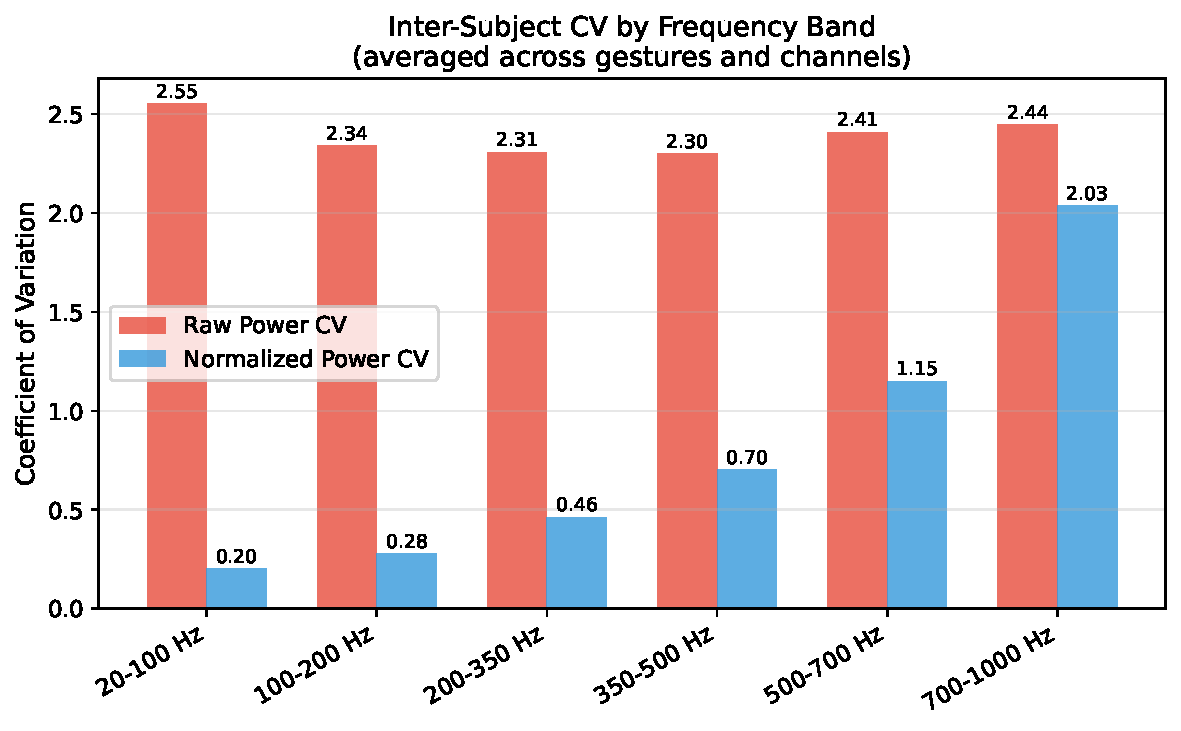
\includegraphics[width=\columnwidth]{fig_h1_cv_by_band.pdf}
\caption{Межсубъектный коэффициент вариации (CV) по частотным полосам, усреднённый по 10~жестам и 12~каналам (40~субъектов). Красный: CV сырой мощности (плоский $\sim$2,3--2,6). Синий: нормированный CV (мощность в полосе / общая мощность) --- \textbf{десятикратный рост} от 20--100\,Гц до 700--1000\,Гц.}
\label{fig:h1_cv}
\end{figure}

\begin{figure}[t]
\centering
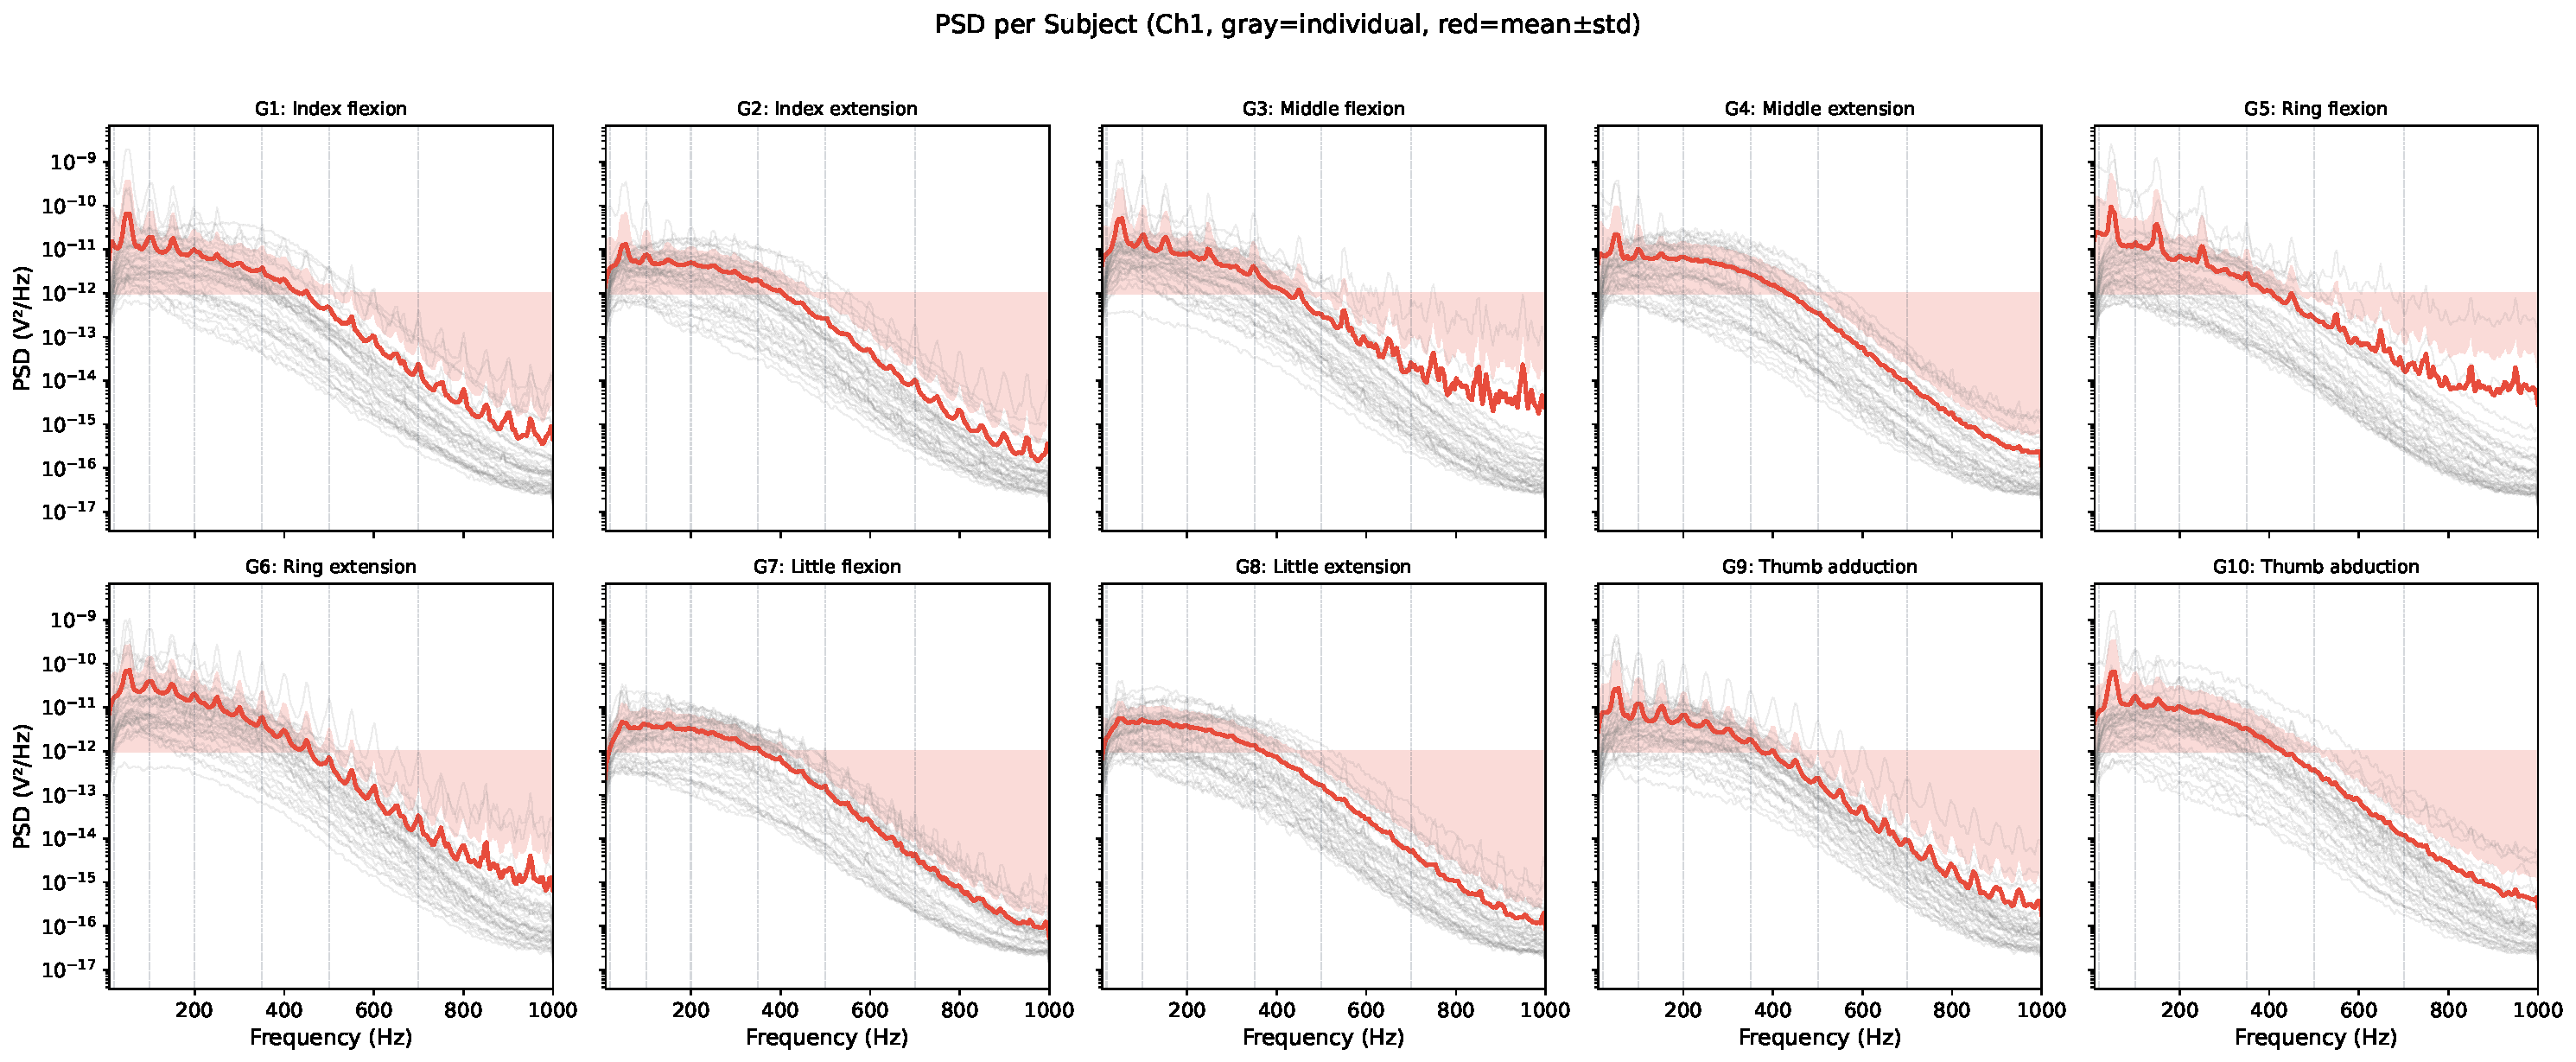
\includegraphics[width=\columnwidth]{fig_h1_psd_overlay.pdf}
\caption{СПМ Уэлча по жестам (канал~1, 40~субъектов). Серые линии --- индивидуальные субъекты; красная --- среднее $\pm$ std. Межсубъектная огибающая расширяется неравномерно по спектру, что мотивирует побандовую обработку.}
\label{fig:h1_psd}
\end{figure}

\Cref{fig:h1_heatmap} детализирует этот паттерн по отдельным жестам: нормированный CV монотонно растёт от нижних к верхним полосам для \emph{каждого} из 10~жестов, что подтверждает универсальность наблюдения.

\begin{figure}[t]
\centering
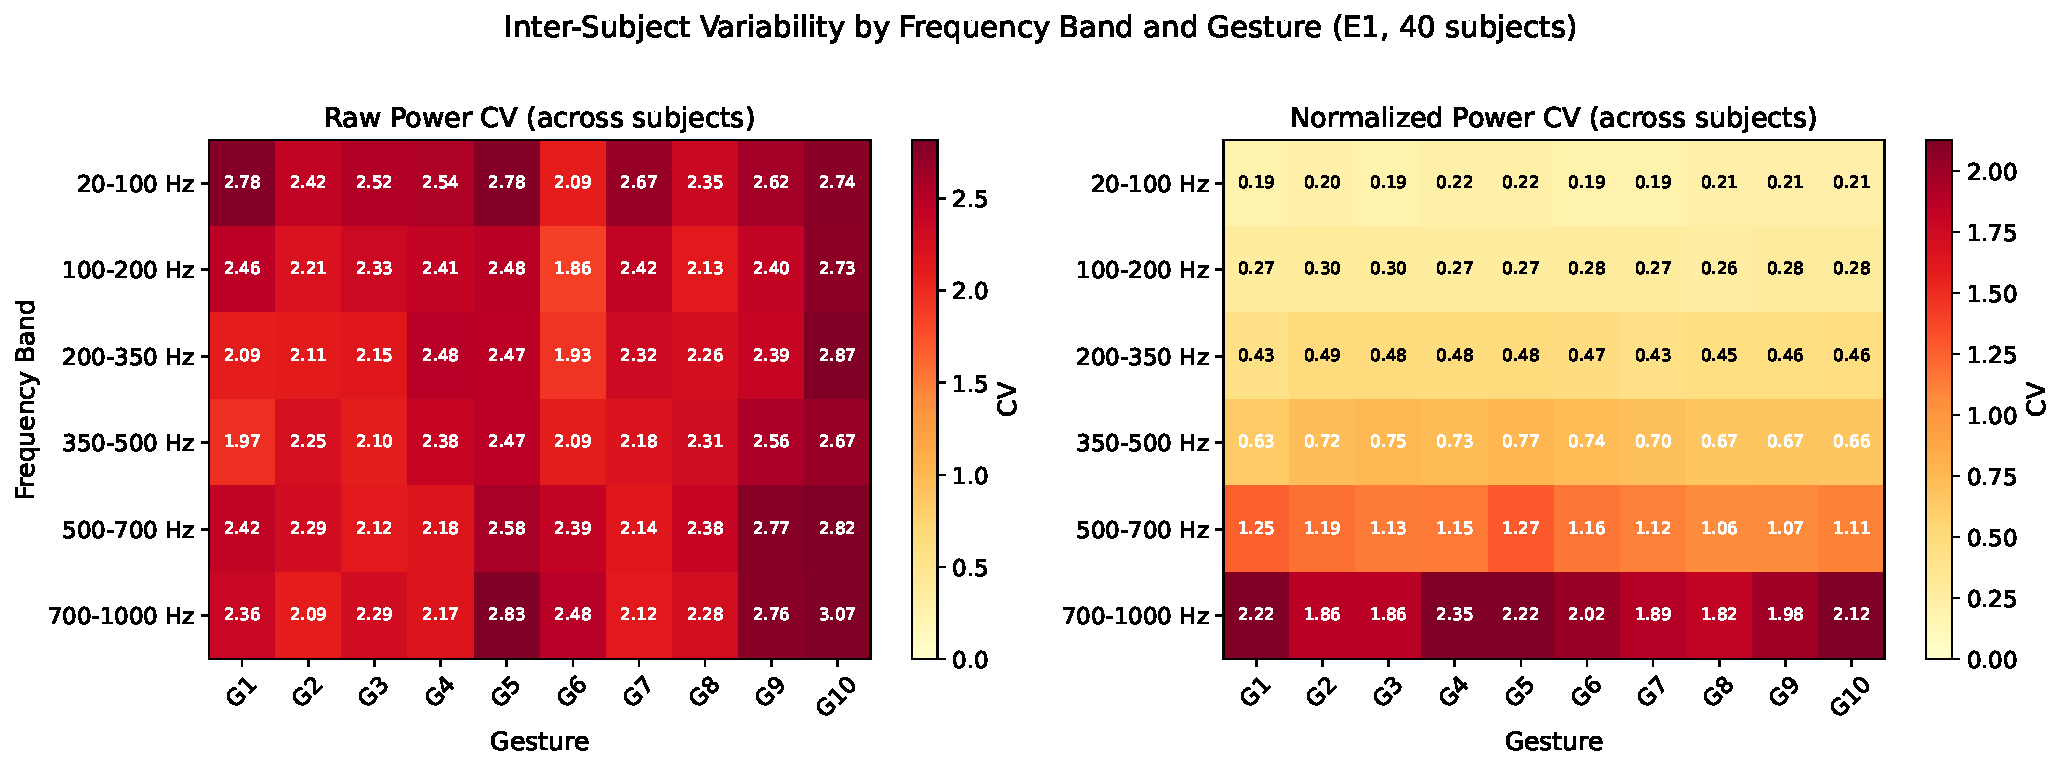
\includegraphics[width=\columnwidth]{fig_h1_cv_heatmap.pdf}
\caption{Тепловая карта межсубъектного CV по частотным полосам и жестам (40~субъектов). Слева: CV сырой мощности (равномерно высокий). Справа: нормированный CV --- монотонный рост от низких частот к высоким для каждого жеста.}
\label{fig:h1_heatmap}
\end{figure}

\textbf{Следствие.} Монолитная модель, обрабатывающая все частоты одинаково, вынуждена искать компромисс между подавлением высокочастотного субъектного шума и сохранением низкочастотной информации о жестах.
Частотная декомпозиция позволяет побандовую обработку, применяя более сильную нормализацию там, где вариабельность максимальна.
В следующем разделе мы описываем конвейер обработки, спроектированный на основе этого наблюдения.

% ======================================================================
%  V. МЕТОД
% ======================================================================
\section{Предлагаемый метод}
\label{sec:method}

\begin{figure}[t]
\centering
\resizebox{\columnwidth}{!}{%
\begin{tikzpicture}[
    >=Stealth,
    node distance=0.45cm and 0.55cm,
    font=\sffamily\scriptsize,
    inputbox/.style={
        rectangle, rounded corners=2pt, draw=black!70, fill=gray!12,
        minimum height=0.7cm, minimum width=1.1cm, align=center,
        line width=0.4pt
    },
    decompbox/.style={
        rectangle, rounded corners=2pt, draw=blue!70!black, fill=blue!12,
        minimum height=0.7cm, minimum width=1.3cm, align=center,
        line width=0.4pt
    },
    mixbox/.style={
        rectangle, rounded corners=2pt, draw=orange!80!black, fill=orange!12,
        minimum height=0.5cm, minimum width=0.9cm, align=center,
        line width=0.4pt
    },
    encbox/.style={
        rectangle, rounded corners=2pt, draw=green!60!black, fill=green!10,
        minimum height=0.5cm, minimum width=1.1cm, align=center,
        line width=0.4pt
    },
    classbox/.style={
        rectangle, rounded corners=2pt, draw=red!70!black, fill=red!10,
        minimum height=0.7cm, minimum width=1.0cm, align=center,
        line width=0.4pt
    },
    concatbox/.style={
        rectangle, rounded corners=2pt, draw=black!60, fill=yellow!8,
        minimum height=0.7cm, minimum width=0.7cm, align=center,
        line width=0.4pt
    },
    arrstyle/.style={->, line width=0.4pt, black!70},
    dimlabel/.style={font=\sffamily\tiny, text=black!60},
]

% ---- Input ----
\node[inputbox] (input) {Input\\$\mathbf{X}$};
\node[dimlabel, below=0.08cm of input] {$400{\times}12$};

% ---- Decomposition ----
\node[decompbox, right=0.7cm of input] (decomp) {Sinc / \textsc{uvmd}\\$K{=}4$ bands};

\draw[arrstyle] (input) -- (decomp);

% ---- Sub-band fan-out: 4 parallel paths ----
\foreach \i/\lab in {1/$X_1$, 2/$X_2$, 3/$X_3$, 4/$X_4$} {
    \pgfmathsetmacro{\yoff}{(2.5 - \i) * 0.72}
    \node[dimlabel, right=0.55cm of decomp, yshift=\yoff cm] (sb\i) {\lab};
}

% Arrows from decomp to sub-band labels
\foreach \i in {1,2,3,4} {
    \draw[arrstyle] (decomp.east) -- (sb\i.west);
}

% ---- MixStyle blocks ----
\foreach \i in {1,2,3,4} {
    \node[mixbox, right=0.25cm of sb\i] (mix\i) {\textsc{Mix}\\Style};
}

\foreach \i in {1,2,3,4} {
    \draw[arrstyle] (sb\i) -- (mix\i);
}

% ---- Dashed "training only" box around MixStyle ----
\begin{scope}[on background layer]
    \node[draw=orange!70!black, dashed, rounded corners=3pt, line width=0.5pt,
          inner sep=3pt, fit=(mix1)(mix4),
          label={[font=\sffamily\tiny, text=orange!70!black]below:training only}] (mixfit) {};
\end{scope}

% ---- Per-band CNN encoders ----
\foreach \i in {1,2,3,4} {
    \node[encbox, right=0.35cm of mix\i] (enc\i) {CNN\\Encoder};
}

\foreach \i in {1,2,3,4} {
    \draw[arrstyle] (mix\i) -- (enc\i);
}

% z_k labels
\foreach \i in {1,2,3,4} {
    \node[dimlabel, above=0.01cm of enc\i, font=\sffamily\tiny] {$\mathbf{z}_\i$};
}

% ---- Concat node ----
\coordinate (encmid) at ($(enc2.east)!0.5!(enc3.east)$);
\node[concatbox, right=0.65cm of encmid] (concat) {$\oplus$};

\foreach \i in {1,2,3,4} {
    \draw[arrstyle] (enc\i.east) -- (concat.west);
}

\node[dimlabel, below=0.08cm of concat] {$\mathbf{z}{\in}\mathbb{R}^{512}$};

% ---- Classifier ----
\node[classbox, right=0.55cm of concat] (cls) {MLP\\$512{\to}256{\to}10$};
\draw[arrstyle] (concat) -- (cls);

% Output
\node[dimlabel, right=0.3cm of cls] (out) {$\hat{y}$};
\draw[arrstyle] (cls) -- (out);

% ---- Encoder detail annotation ----
\node[font=\sffamily\tiny, text=green!50!black, below=0.35cm of enc4,
      align=center, anchor=north]
      {Conv64--BN--ReLU\\Conv128--BN--ReLU\\AvgPool $\to$ $\mathbb{R}^{128}$};

% ---- Stage labels (top) ----
\node[font=\sffamily\tiny\bfseries, text=gray!70, above=0.45cm of decomp] {Stage 1};
\node[font=\sffamily\tiny\bfseries, text=gray!70, above=0.45cm of mixfit] {Stage 2};
\node[font=\sffamily\tiny\bfseries, text=gray!70, above=0.45cm of enc1] {Stage 3};
\node[font=\sffamily\tiny\bfseries, text=gray!70, above=0.45cm of cls] {Stage 4};

\end{tikzpicture}%
}% end resizebox
\iflanguage{russian}{%
\caption{Архитектура предлагаемого частотно-ориентированного конвейера.
Этап~1: декомпозиция входного сигнала на $K{=}4$ частотных поддиапазона (Sinc или \textsc{uvmd}).
Этап~2: побандовый \textsc{MixStyle} (только при обучении; ноль параметров) смешивает статистики между субъектами.
Этап~3: независимое кодирование каждого поддиапазона CNN-энкодером ($\mathbf{z}_k \in \mathbb{R}^{128}$).
Этап~4: классификация конкатенированного представления $\mathbf{z} \in \mathbb{R}^{512}$ MLP-головой.}%
}{%
\caption{Architecture of the proposed frequency-aware sEMG pipeline.
Stage~1 decomposes the raw input into $K{=}4$ frequency sub-bands via either
a fixed Sinc filterbank or learnable \textsc{uvmd}.
Stage~2 applies per-band \textsc{MixStyle} (training only; zero parameters) to
mix channel-wise statistics between subjects.
Stage~3 encodes each sub-band independently through shared-architecture CNN
encoders, producing $\mathbf{z}_k \in \mathbb{R}^{128}$.
The concatenated representation $\mathbf{z} \in \mathbb{R}^{512}$ is classified
by an MLP head (Stage~4).}%
}
\label{fig:architecture}
\end{figure}


Наш конвейер (\cref{fig:architecture}) обрабатывает окно необработанного пЭМГ $\mathbf{X} \in \mathbb{R}^{T \times C}$ ($T$\,=\,400 отсчётов, $C$\,=\,12 каналов) в четыре этапа:

\subsection{Этап 1: Частотная декомпозиция}
Мы декомпозируем $\mathbf{X}$ на $K$\,=\,4 поддиапазонных сигнала $\{\mathbf{X}_k\}_{k=1}^{K}$, каждый $\in \mathbb{R}^{T \times C}$, используя один из двух фронтендов:

\paragraph{Фиксированный Sinc-фильтрбанк.}
Четыре полосовых Sinc-фильтра с фиксированными частотами среза разбивают полосу Найквиста на равные поддиапазоны.
Для фильтра $k$ с полосой пропускания $[f_k^{\mathrm{lo}}, f_k^{\mathrm{hi}}]$:
\begin{equation}
h_k[n] = 2f_k^{\mathrm{hi}} \operatorname{sinc}(2f_k^{\mathrm{hi}} n) - 2f_k^{\mathrm{lo}} \operatorname{sinc}(2f_k^{\mathrm{lo}} n)
\label{eq:sinc}
\end{equation}
с окном Хэмминга, применяемая свёрткой к каждому каналу независимо.
Частоты среза фиксированы: $[0; 0{,}125; 0{,}25; 0{,}375; 0{,}5]$ (нормированная частота), что соответствует четырём равным полосам.
Фронтенд добавляет только 8 параметров.

\paragraph{Развёрнутый VMD (\uvmd{}).}
Мы \emph{разворачиваем} $L$\,=\,8 итераций ADMM-обновления для VMD~\cite{dragomiretskiy2014variational} в дифференцируемый нейросетевой блок.
Обучаемые параметры:
\begin{itemize}
    \item $\boldsymbol{\alpha} \in \mathbb{R}^{L \times K}$: штраф на полосу пропускания (по итерациям и модам),
    \item $\boldsymbol{\tau} \in \mathbb{R}^{L}$: шаг Лагранжиана (по итерациям),
    \item $\boldsymbol{\omega} \in \mathbb{R}^{K}$: центральные частоты (инициализированы равномерно: $[0{,}05; 0{,}18; 0{,}32; 0{,}45]$).
\end{itemize}
На каждой ADMM-итерации $l$ для моды $k$ спектральное обновление:
\begin{equation}
\hat{u}_k^{(l)}(\xi) = \frac{\hat{r}_k(\xi)}{1 + \alpha_{l,k} (\xi - \omega_k)^2}
\label{eq:uvmd}
\end{equation}
где $\hat{r}_k$~--- остаток после удаления всех остальных мод.
Штраф на спектральное перекрытие $\mathcal{L}_{\mathrm{overlap}} = \sum_{j \neq k} \exp(-10(\omega_j - \omega_k)^2)$ стимулирует частотное разнообразие.
Фронтенд добавляет 44 параметра ($\boldsymbol{\alpha}$: 32, $\boldsymbol{\tau}$: 8, $\boldsymbol{\omega}$: 4).

\subsection{Этап 2: Побандовый энкодер}
Каждый поддиапазон $\mathbf{X}_k$ независимо кодируется 1D-CNN с общей архитектурой:
\begin{multline}
\mathbf{z}_k = \operatorname{AvgPool}\!\big(\operatorname{ReLU}\!\big(\operatorname{BN}\!\big( \\
\operatorname{Conv}_{128}\!\big(\operatorname{ReLU}\!\big(\operatorname{BN}\!\big(\operatorname{Conv}_{64}(\mathbf{X}_k)\big)\big)\big)\big)\big)\big)
\end{multline}
где $\operatorname{Conv}_{d}$ обозначает $\operatorname{Conv1d}(C, d, \cdot)$ с ядрами 5 и 3 соответственно, а $\operatorname{AvgPool}$~--- глобальное адаптивное среднее.
Каждый энкодер отображает $\mathbb{R}^{T \times C} \to \mathbb{R}^{128}$; четыре энкодера дают $\mathbf{z} = [\mathbf{z}_1; \ldots; \mathbf{z}_4] \in \mathbb{R}^{512}$.

\subsection{Этап 3: Побандовый \mixstyle{}}
\label{sec:mixstyle}
Только при обучении мы применяем \mixstyle{}~\cite{zhou2021mixstyle} независимо к каждому поддиапазону \emph{до} кодирования.
Для поддиапазона $k$ и образца $i$ в мини-батче:
\begin{align}
\mu_k^{(i)} &= \mathbb{E}_t[\mathbf{X}_k^{(i)}], \quad
\sigma_k^{(i)} = \sqrt{\operatorname{Var}_t[\mathbf{X}_k^{(i)}] + \epsilon} \label{eq:ms_stats} \\
\tilde{\mathbf{X}}_k^{(i)} &= \frac{\mathbf{X}_k^{(i)} - \mu_k^{(i)}}{\sigma_k^{(i)}} \label{eq:ms_norm} \\
\lambda &\sim \operatorname{Beta}(\alpha, \alpha), \quad j = \operatorname{shuffle}(i) \label{eq:ms_lambda} \\
\tilde{\mu}_k &= \lambda \mu_k^{(i)} + (1-\lambda) \mu_k^{(j)}, \quad
\tilde{\sigma}_k = \lambda \sigma_k^{(i)} + (1-\lambda) \sigma_k^{(j)} \label{eq:ms_mix} \\
\hat{\mathbf{X}}_k^{(i)} &= \tilde{\sigma}_k \cdot \tilde{\mathbf{X}}_k^{(i)} + \tilde{\mu}_k \label{eq:ms_out}
\end{align}
с $\alpha$\,=\,0,1 и вероятностью применения $p$\,=\,0,5.
Этот модуль имеет \textbf{ноль обучаемых параметров}: он только манипулирует статистиками.
Ключевое отличие от глобального \mixstyle{}~--- побандовое применение, позволяющее разные уровни стилевых возмущений в каждом частотном диапазоне.

\paragraph{Адаптивный побандовый \mixstyle{} (H8).}
Мы расширяем фиксированный модуль, делая $\alpha$ и $p$ \emph{обучаемыми для каждой полосы}:
\begin{equation}
\alpha_k = \operatorname{softplus}(\theta_k^{\alpha}) + \epsilon, \quad
p_k = \sigma(\theta_k^{p})
\label{eq:adaptive_ms}
\end{equation}
где $\theta_k^{\alpha}, \theta_k^{p}$~--- необработанные параметры, инициализированные для $\alpha_k$\,=\,0,1, $p_k$\,=\,0,5.
Выход~--- мягкое смешивание оригинала и стилизованного сигнала:
$\hat{\mathbf{X}}_k = p_k \cdot \tilde{\mathbf{X}}_k^{\mathrm{mixed}} + (1 - p_k) \cdot \mathbf{X}_k$,
что обеспечивает полную дифференцируемость через репараметризованную выборку из Beta-распределения.
Это добавляет всего $2K$\,=\,8 обучаемых параметров.

\paragraph{Spectral Content Gate (H9).}
Вместо аугментации стиля (MixStyle), \emph{Spectral Content Gate} (SCG) обучается его \emph{селективному удалению}. Для каждой полосы $k$ обучаемый гейт $\gamma_k = \sigma(\theta_k^{\gamma}) \in [0, 1]$ смешивает нормализованный (без стиля) и исходный (со стилем) вход:
\begin{equation}
\hat{\mathbf{X}}_k = \gamma_k \cdot \frac{\mathbf{X}_k - \mu_k}{\sigma_k} + (1 - \gamma_k) \cdot \mathbf{X}_k
\label{eq:scg}
\end{equation}
При $\gamma_k \to 1$ полоса $k$ проходит полную Instance Normalization; при $\gamma_k \to 0$ исходный сигнал сохраняется. Это добавляет всего $K$\,=\,4 обучаемых параметра. Ключевое отличие от MixStyle: SCG~--- \emph{детерминистический модуль, активный при инференсе}, а не обучающая аугментация.

\subsection{Этап 4: Классификатор}
Двуслойный MLP отображает $\mathbf{z} \in \mathbb{R}^{512}$ в логиты классов:
$512 \to 256$ (ReLU, dropout $p$\,=\,0,3) $\to$ 10 (softmax).

\paragraph{Обучение.}
Суммарная функция потерь:
\begin{equation}
\mathcal{L} = \mathcal{L}_{\mathrm{CE}} + \lambda_{\mathrm{ov}} \cdot \mathcal{L}_{\mathrm{overlap}}
\end{equation}
с $\lambda_{\mathrm{ov}}$\,=\,0,01 (только для \uvmd{}; ноль для Sinc).
Используется Adam ($\mathrm{lr}$\,=\,$10^{-3}$), ReduceLROnPlateau (фактор 0,5, терпение 5) и ранняя остановка (терпение 15) до 80~эпох.

\paragraph{Размер модели.}
\Cref{tab:params} суммирует число параметров.
Фронтенд декомпозиции добавляет пренебрежимо мало (8--44 параметра); основные затраты~--- четыре побандовых энкодера (116\,000).
\mixstyle{} добавляет ноль параметров.

\begin{table}[t]
\centering
\caption{Число параметров по вариантам модели.}
\label{tab:params}
\resizebox{\columnwidth}{!}{%
\begin{tabular}{lrrl}
\toprule
Вариант & Всего & Фронтенд & Примечание \\
\midrule
A: Raw CNN ($K$=1) & 64\,586 & 0 & Один энкодер \\
B: Sinc FB ($K$=4) & 249\,874 & 8 & 4 энкодера \\
C: Sinc + \mixstyle{} & 249\,874 & 8 & +0 для \mixstyle{} \\
D: Sinc + MS + CS & 172\,130 & 8 & Контент/стиль \\
E/F: \uvmd{} ($K$=4) & 249\,910 & 44 & Обучаемая декомп. \\
G: Sinc + Адапт. MS & 249\,882 & 16 & +8 для $\alpha_k, p_k$ \\
H: \uvmd{} + Адапт. MS & 249\,918 & 52 & +8 для $\alpha_k, p_k$ \\
SCG-A: Sinc + SCG & 136\,974 & 12 & +4 для $\gamma_k$ \\
SCG-B: \uvmd{} + SCG + Адв & 172\,365 & 48 & +4 $\gamma_k$, +35K адв. \\
\bottomrule
\end{tabular}%
}
\end{table}

% ======================================================================
%  VI. ЭКСПЕРИМЕНТЫ И РЕЗУЛЬТАТЫ
% ======================================================================
\section{Эксперименты и результаты}
\label{sec:results}

Экспериментальная оценка строится вокруг центрального противопоставления: \emph{глобальная} инвариантность (удаление стиля из всех частот, состязательное разделение) vs. \emph{частотно-селективная} обработка (декомпозиция + побандовая аугментация).
Мы сначала показываем, что глобальные подходы вредят (\cref{sec:negative}), затем количественно оцениваем вклад каждого компонента частотно-селективного конвейера (\cref{sec:h6}), и наконец проверяем, обучается ли сеть частотному градиенту вариабельности самостоятельно (\cref{sec:h8,sec:h9}).
\Cref{tab:hypotheses} суммирует все проверенные гипотезы; статистические детали~--- в~\cref{sec:stats}.

\begin{table*}[t]
\centering
\caption{Сводка цепочки гипотез. NinaPro DB2 E1, 20 субъектов, строгий LOSO. $p_{\mathrm{Холм}}$: скорректировано внутри семейства гипотез. Статус: \textbf{К}~=~конфирматорный ($p_{\mathrm{Холм}}$\,$<$\,0,05), \textbf{Р}~=~разведочный (только $p_{\mathrm{нескорр.}}$\,$<$\,0,05), \textbf{О}~=~отвергнут, \textbf{Д}~=~дескриптивный. Метки семейств: A=декомпозиция, B=мягкий стиль, C=жёсткая норм., D=разделение, E=SCG-Net. $\dagger$H2--H4: batch=64; H6--H9: batch=512 (см. \cref{sec:batchsize}).}
\label{tab:hypotheses}
\begin{tabular}{clp{4.8cm}ccccc}
\toprule
\# & Гипотеза & Ключевой вопрос & Семейство & Статус & $\Delta$F1 & $p_{\mathrm{нескорр.}}$ & $p_{\mathrm{Холм}}$ \\
\midrule
H1 & Спектр. вариаб. & Зависит ли межсубъектная вариабельность от частоты? & --- & \textbf{Д} & --- & --- & --- \\
H2$^\dagger$ & Декомпозиция & Превосходит ли декомпозиция необработанный сигнал? & A & \textbf{К} & +2,3\pp{} & 0,007 & $<$0,02 \\
H3$^\dagger$ & Стилевая норм. & Помогает ли побандовый \mixstyle{}? & B & \textbf{Р} & +1,7\pp{} & 0,04 & 0,08 \\
   &                 & Помогает ли Instance Norm? & C & \textbf{О (К)} & $-$7,0\pp{} & $<$0,001 & $<$0,002 \\
H4$^\dagger$ & Разделение & Помогает ли явное разделение контент/стиль? & D & \textbf{О (К)} & $-$2,6\pp{} & $<$0,001 & $<$0,004 \\
H6 & Абляция & Вклад декомпозиции (A$\to$B) & A & \textbf{К} & +3,7\pp{} & $<$0,001 & $<$0,003 \\
   &         & Вклад \mixstyle{} (B$\to$C) & B & \textbf{Р} & +1,1\pp{} & 0,07 & 0,07 \\
H7 & \uvmd{}+\mixstyle{} & Агностичен ли \mixstyle{} к фронтенду? & B & \textbf{К} & +1,8\pp{} & 0,003 & $<$0,01 \\
H8 & Адапт. \mixstyle{} & Обучается ли сеть градиенту H1? & --- & \textbf{Д$^{\ddagger}$} & +0,97\pp{} & 0,064 & --- \\
H9 & SCG-Net & Превосходит ли побандовый гейт равномерную IN? & E & \textbf{К} & +6,86\pp{} & $<$0,001 & $<$0,001 \\
\bottomrule
\multicolumn{8}{l}{\footnotesize $\ddagger$Статус H8~--- Д (дескриптивный): основное свидетельство~--- градиент обученных параметров (Spearman $\rho$\,=\,0,78), а не $\Delta$F1.} \\
\multicolumn{8}{l}{\footnotesize Дополнительно проверено увеличение числа полос ($K$\,=\,6, 8), SE-attention, GroupDRO~--- без значимых улучшений (Фридман $p$\,=\,0,71).}
\end{tabular}
\end{table*}

\subsection{H2: Частотная декомпозиция vs. необработанный сигнал}

\Cref{tab:h2} показывает, что декомпозиция на $K$\,=\,4 полосы устойчиво превосходит обработку необработанного сигнала.
Sinc-фильтрбанк и \uvmd{} дают +2,1--2,3\pp{} F1 со средним размером эффекта ($d$\,$\approx$\,0,67--0,68).
В рамках Семейства~A (декомпозиция, $k$\,=\,3) оба сравнения достигают значимости после поправки Холма ($p_{\mathrm{Холм}}$\,$<$\,0,02), а контролируемая абляция H6~(\cref{sec:h6}) независимо подтверждает эффект ($p_{\mathrm{Холм}}$\,$<$\,0,003).
Sinc и \uvmd{} статистически неразличимы ($\Delta$\,=\,+0,24\pp{}, $p$\,=\,0,50), что мотивирует использование более простого Sinc-фронтенда в последующих экспериментах.

\emph{Примечание:} ранние и поздние серии экспериментов различаются размером батча (64 vs. 512); абсолютные F1 между таблицами не сопоставимы напрямую (см.~\cref{sec:batchsize}).

\begin{table}[t]
\centering
\caption{H2: Сравнение декомпозиций (20 субъектов, LOSO).}
\label{tab:h2}
\begin{tabular}{lccc}
\toprule
Фронтенд & F1 (\%) & $\Delta$ vs. raw & $d$ \\
\midrule
Без (raw) & 34,90 $\pm$ 8,16 & --- & --- \\
Sinc FB ($K$=4) & 37,00 $\pm$ 7,56 & +2,10 & 0,67 \\
\uvmd{} ($K$=4) & 37,24 $\pm$ 7,75 & +2,34 & 0,68 \\
\bottomrule
\end{tabular}
\end{table}

\subsection{H3: Побандовая стилевая нормализация}

Установив, что декомпозиция помогает, мы проверяем, можно ли дополнительно улучшить качество побандовой нормализацией стилей.
\Cref{tab:h3} обнаруживает выраженную асимметрию: \emph{мягкая} нормализация (MixStyle) даёт +1,67\pp{} ($d$\,=\,0,54, разведочный), тогда как \emph{жёсткая} (Instance Normalization) катастрофически ухудшает качество: $-$7,0\pp{} для глобальной IN ($d$\,=\,$-$1,13) и $-$8,5\pp{} для побандовой ($d$\,=\,$-$1,36), оба $p_{\mathrm{Холм}}$\,$<$\,0,002.

Адаптивный вариант IN, обучающий силу нормализации $\gamma_k$ для каждой полосы, даёт ценную диагностику: он сходится к $\gamma_1$\,=\,0,027 (низкие частоты) против $\gamma_4$\,=\,0,38 (высокие частоты)~--- \textbf{соотношение 14:1}, независимо подтверждающее вывод H1.

\begin{table}[t]
\centering
\caption{H3: Сравнение стилевой нормализации (20 субъектов, LOSO). Бейзлайн: Sinc FB ($K$=4), без нормализации.}
\label{tab:h3}
\begin{tabular}{lccc}
\toprule
Нормализация & F1 (\%) & $\Delta$ & $d$ \\
\midrule
Без (бейзлайн) & 36,28 $\pm$ 7,81 & --- & --- \\
Побандовый \mixstyle{} & \textbf{37,95 $\pm$ 7,22} & +1,67 & 0,54 \\
Адаптивная IN ($\gamma_k$) & 36,90 $\pm$ 6,98 & +0,62 & 0,24 \\
Глобальная IN & 29,29 $\pm$ 5,30 & $-$6,99 & $-$1,13 \\
Побандовая IN & 27,75 $\pm$ 4,29 & $-$8,53 & $-$1,36 \\
\bottomrule
\end{tabular}
\end{table}

\subsection{Отрицательные результаты: что не работает}
\label{sec:negative}

Прежде чем перейти к основной абляции, мы суммируем ключевые отрицательные результаты, определившие направление исследования.

\paragraph{Жёсткая Instance Normalization вредит (\cref{tab:h3}).}
Глобальная IN теряет $-$7,0\pp{} ($p_{\mathrm{Холм}}$\,$<$\,0,002), побандовая IN~--- $-$8,5\pp{}.
IN удаляет \emph{все} статистики первого и второго порядка, включая поканальные амплитудные паттерны, несущие информацию о жесте.

\paragraph{Явное разделение контента и стиля вредит (\cref{tab:h4}).}
Добавление состязательной (GRL), MI-минимизирующей или контрастивной потерь для разделения контента и стиля ухудшает качество на $-$2,6 -- $-$4,3\pp{} ($p_{\mathrm{Холм}}$\,$<$\,0,01).
Состязательная потеря ухудшает \emph{каждого} субъекта (0/20 улучшений, $d$\,=\,$-$2,16).
В нашей постановке контент жеста и стиль субъекта содержат достаточно общей информации; принудительное их разделение разрушает представление.

\begin{table}[t]
\centering
\caption{Влияние вспомогательных потерь разделения контента/стиля (20 субъектов). Бейзлайн: Sinc FB + \mixstyle{} + CS-головы.}
\label{tab:h4}
\resizebox{\columnwidth}{!}{%
\begin{tabular}{lcccc}
\toprule
Потеря & F1 (\%) & $\Delta$ & $d$ & $p_{\mathrm{Холм}}$ \\
\midrule
Без (бейзлайн) & \textbf{39,19 $\pm$ 6,34} & --- & --- & --- \\
+ Контрастивная & 38,99 $\pm$ 5,95 & $-$0,19 & $-$0,14 & 1,00 \\
+ Состязательная (GRL) & 36,60 $\pm$ 5,99 & $-$2,58 & $-$2,16 & $<$0,004 \\
+ MI-минимизация & 35,29 $\pm$ 7,28 & $-$3,89 & $-$0,97 & $<$0,01 \\
+ Все вместе & 34,89 $\pm$ 7,18 & $-$4,30 & $-$1,04 & $<$0,01 \\
\bottomrule
\end{tabular}%
}
\end{table}

\paragraph{Усложнение архитектуры не помогает.}
Увеличение числа полос ($K$\,=\,6, 8), добавление SE-attention и GroupDRO не улучшают качество: критерий Фридмана по шести вариантам $\chi^2$\,=\,2,94, $p$\,=\,0,71.
Простейшая архитектура ($K$\,=\,4, без дополнений) остаётся лучшей.

Эти результаты определили конструкцию итогового конвейера: \emph{неявная} стилевая робастность через \mixstyle{} предпочтительнее \emph{явного} разделения, а $K$\,=\,4 достаточно.

\subsection{Единая абляция (чистая атрибуция компонентов)}
\label{sec:h6}

Для изоляции вкладов отдельных компонентов мы фиксируем единую архитектуру и варьируем один компонент за шаг (\cref{tab:h6}).
Серия абляции использует batch\_size\,=\,512, что влияет на абсолютные значения F1 по сравнению с ранними экспериментами (bs=64); см. \cref{sec:batchsize}.

\begin{table}[t]
\centering
\caption{H6: Единая абляция (20 субъектов, batch=512, LOSO). Каждый шаг добавляет ровно один компонент. Стат. тесты: Уилкоксон с поправкой Холма внутри семейств гипотез (A, B).}
\label{tab:h6}
\resizebox{\columnwidth}{!}{%
\begin{tabular}{llcccccc}
\toprule
& Компоненты & F1 (\%) & IQR & $\Delta_{\mathrm{шаг}}$ & $d$ & $p_{\mathrm{Холм}}$ & $\uparrow/\downarrow$ \\
\midrule
A & Raw CNN & 32,40 $\pm$ 5,91 & 8,9 & --- & --- & --- & --- \\
B & + Sinc FB & 36,08 $\pm$ 7,29 & 10,4 & +3,68 & 1,25 & $<$0,003 & 18/2 \\
C & + \mixstyle{} & \textbf{37,19 $\pm$ 6,21} & 8,5 & +1,11 & 0,42 & 0,07$^*$ & 18/2 \\
D & + CS-головы & 36,37 $\pm$ 6,07 & 8,8 & $-$0,82 & $-$0,62 & 0,34 & 5/15 \\
\bottomrule
\multicolumn{8}{l}{\footnotesize $^*$Разведочный: не достигает значимости в рамках Семейства~B.}
\end{tabular}%
}
\end{table}

Абляция подтверждает, что частотная декомпозиция~--- наибольший отдельный вклад в конвейер: она добавляет +3,7\pp{} с большим размером эффекта (\cref{tab:h6}).
Побандовый \mixstyle{} добавляет ещё +1,1\pp{}; направление устойчиво (18 из 20 субъектов улучшаются), но индивидуально не достигает значимости после поправки.
Добавление контент/стиль голов ухудшает качество, что согласуется с отрицательными результатами явного разделения (\cref{sec:negative}).
Итог: лучший вариант~--- Sinc + побандовый \mixstyle{} (\cref{fig:ablation_bar}).

\begin{figure}[t]
\centering
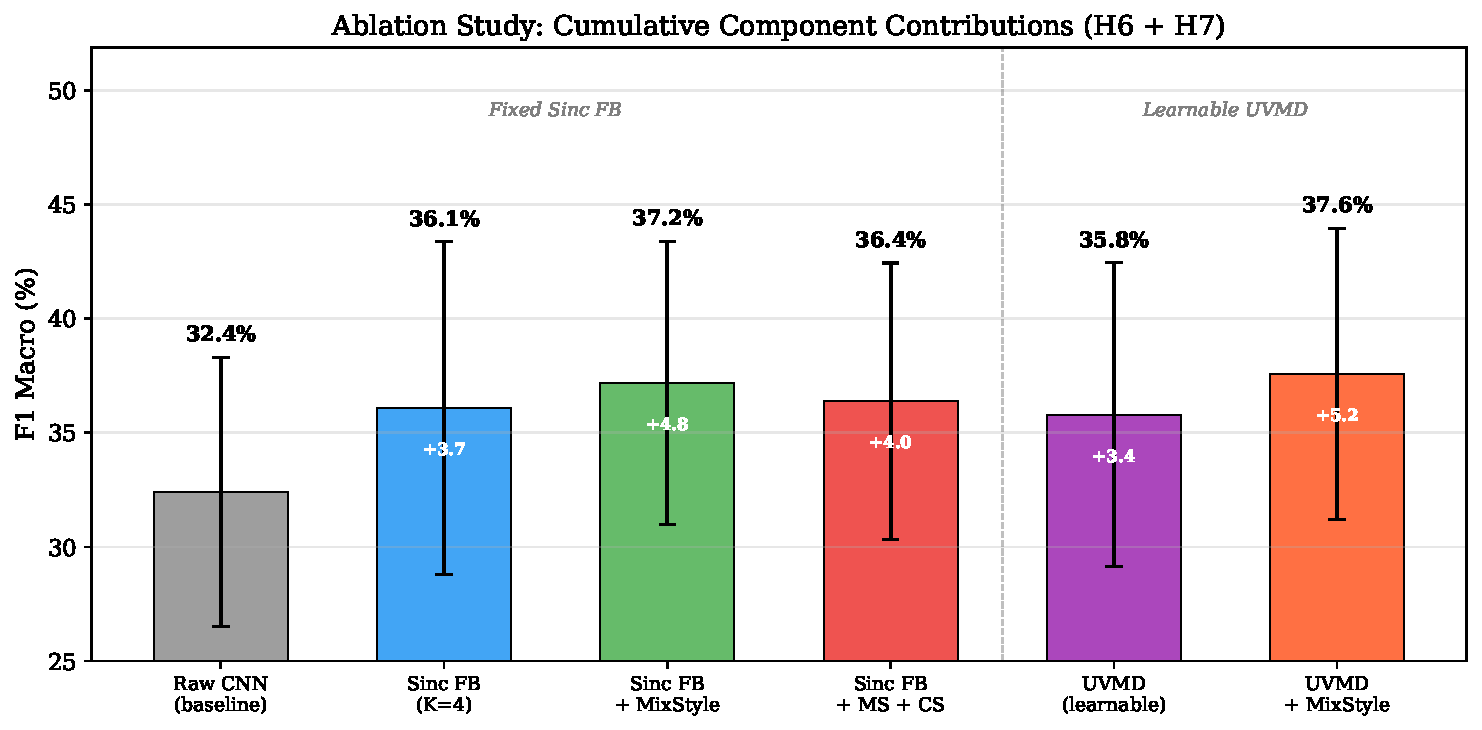
\includegraphics[width=\columnwidth]{fig_h6h7_ablation.pdf}
\caption{Вклад компонентов конвейера (абляция H6~+~H7). Слева: фиксированный Sinc-фронтенд; справа: обучаемый \uvmd{}. Числа внутри столбцов --- суммарное улучшение над бейзлайном Raw CNN. Декомпозиция вносит наибольший вклад (+3,4--3,7\pp{}); \mixstyle{} добавляет дополнительные +1,1--1,8\pp{}.}
\label{fig:ablation_bar}
\end{figure}

\subsection{H7: Универсальность побандового \mixstyle{}}

Помогает ли \mixstyle{} только с фиксированной декомпозицией, или он \emph{агностичен к фронтенду}?
Проверяем на обучаемом \uvmd{} (\cref{tab:h7}).

\begin{table}[t]
\centering
\caption{H7: \uvmd{} + \mixstyle{} (20 субъектов, batch=512, LOSO; вариант~F воспроизведён при batch=64, $p$\,=\,0,67). E$\to$F: $p_{\mathrm{Холм}}$\,$<$\,0,01 (Семейство~B, конфирматорный).}
\label{tab:h7}
\resizebox{\columnwidth}{!}{%
\begin{tabular}{llcccc}
\toprule
& Фронтенд + стиль & F1 (\%) & $\Delta$ & $d$ & $p_{\mathrm{нескорр.}}$ \\
\midrule
E & \uvmd{} & 35,79 $\pm$ 6,67 & --- & --- & --- \\
F & \uvmd{} + \mixstyle{} & \textbf{37,58 $\pm$ 6,39} & +1,79 & 0,84 & 0,003 \\
\midrule
& \multicolumn{5}{l}{\textit{Сравнение фронтендов:}} \\
B & Sinc FB & 36,08 $\pm$ 7,29 & \multirow{2}{*}{---} & \multirow{2}{*}{$-$0,16} & \multirow{2}{*}{0,78} \\
E & \uvmd{} & 35,79 $\pm$ 6,67 & & & \\
C & Sinc + MS & 37,19 $\pm$ 6,21 & \multirow{2}{*}{+0,39} & \multirow{2}{*}{0,25} & \multirow{2}{*}{0,43} \\
F & \uvmd{} + MS & 37,58 $\pm$ 6,39 & & & \\
\bottomrule
\end{tabular}%
}
\end{table}

На обучаемом \uvmd{}-фронтенде побандовый \mixstyle{} добавляет +1,8\pp{} с большим размером эффекта ($d$\,=\,0,84), и этот результат является \textbf{конфирматорным} после поправки Холма (\cref{tab:h7}).
На фиксированном Sinc эффект устойчив по направлению (+1,1\pp{}, 18/20 субъектов), но остаётся разведочным.
Это различие может объясняться тем, что адаптивное размещение частот \uvmd{} создаёт поддиапазоны, в которых статистики стилей более информативны.

Два фронтенда статистически неразличимы по итоговому F1: разница минимальна, а выбор между ними не влияет на основной вывод.
Воспроизведение лучшего варианта при batch\_size\,=\,64 подтверждает робастность: результат не меняется ($p$\,=\,0,67; см.~\cref{sec:batchsize}).

\begin{figure*}[t]
\centering
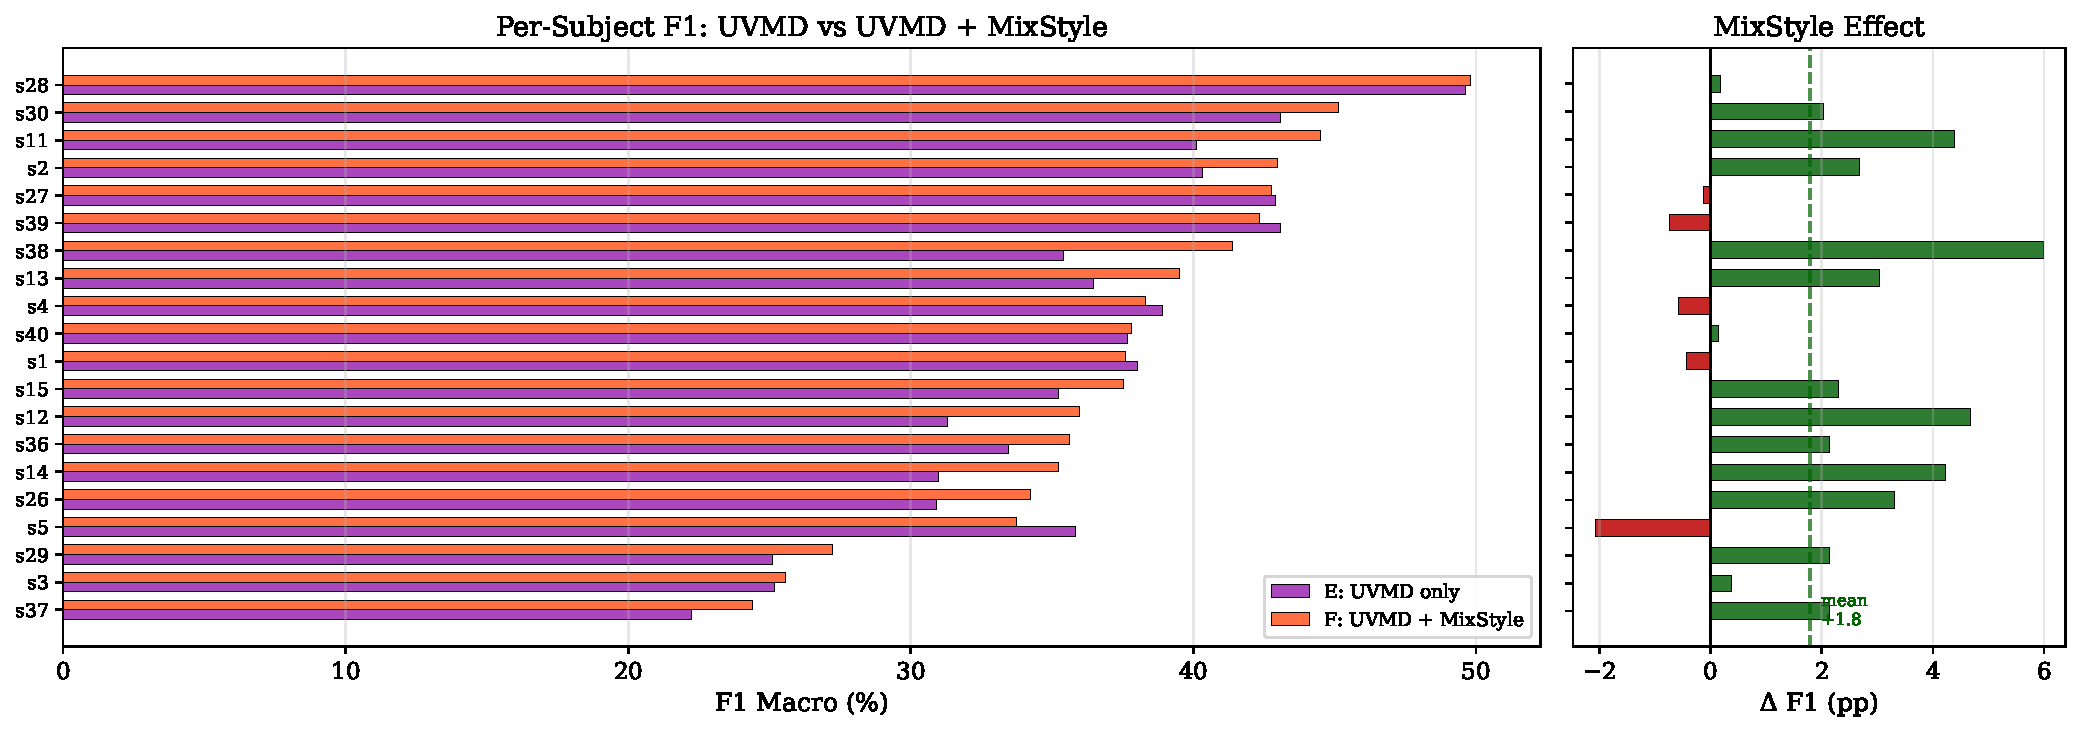
\includegraphics[width=\textwidth]{fig_h7_per_subject.pdf}
\caption{Пер-субъектный F1 для \uvmd{} (фиолетовый) и \uvmd{}+\mixstyle{} (оранжевый), отсортирован по убыванию F1 (слева). Справа: пер-субъектный прирост $\Delta$F1 от \mixstyle{}. 16 из 20 субъектов получают положительный прирост (зелёные столбцы), средний эффект +1,8\pp{}.}
\label{fig:h7_per_subject}
\end{figure*}

\paragraph{Обученные частоты \uvmd{}.}
\Cref{fig:omega_psd} показывает обученные центральные частоты, наложенные на спектр мощности ЭМГ.
Начиная с равномерной инициализации [100, 367, 633, 900]\,Гц, \uvmd{} сходится к [87$\pm$4, 385$\pm$4, 671$\pm$4, 889$\pm$9]\,Гц по всем 20~субъектам (std\,$<$\,10\,Гц), указывая на \emph{универсальную}, субъект-независимую частотную декомпозицию.

\begin{figure}[t]
\centering
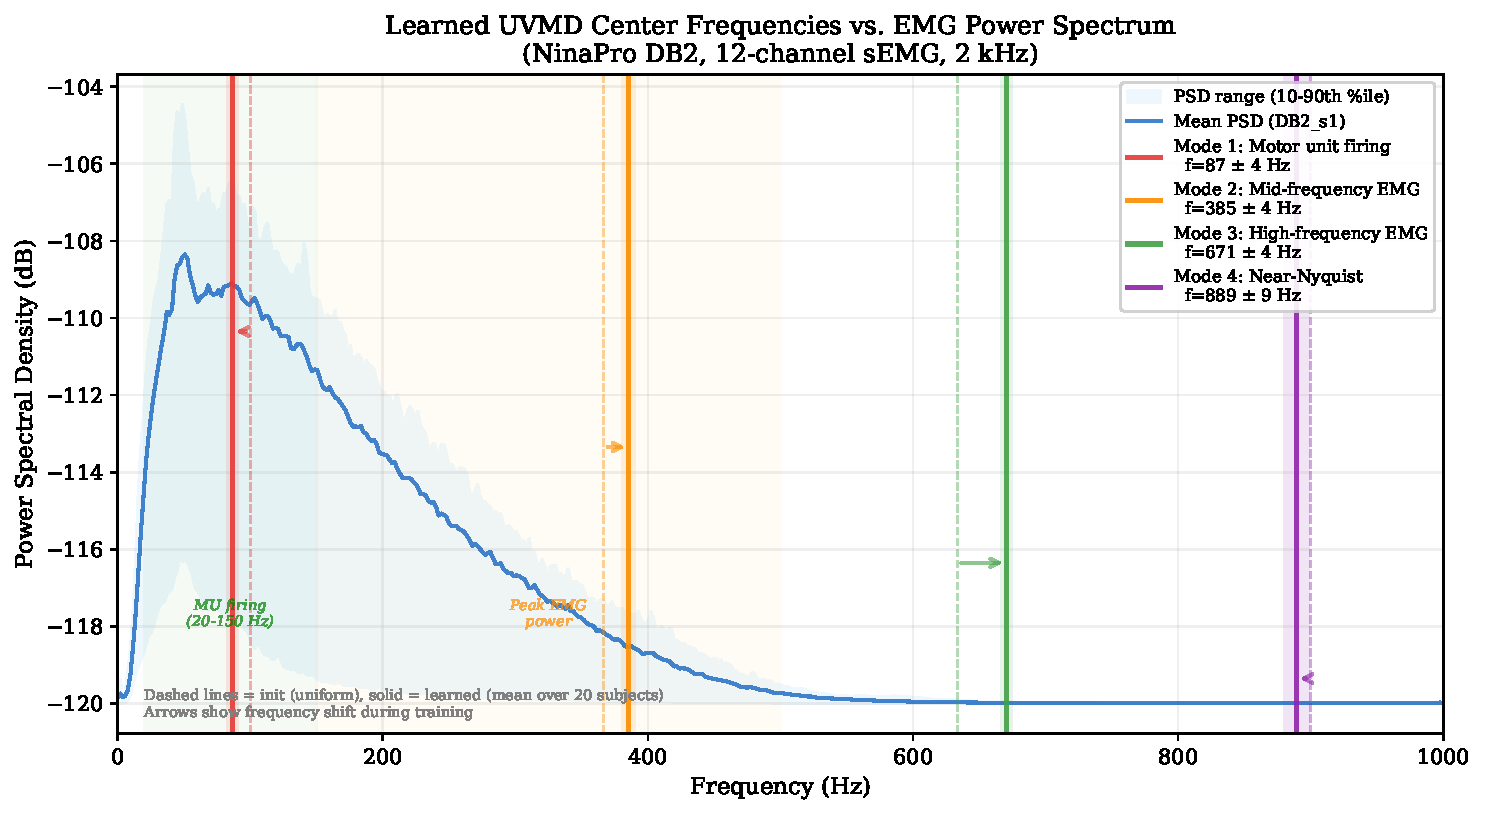
\includegraphics[width=\columnwidth]{fig_uvmd_omega_psd.pdf}
\caption{Обученные центральные частоты \uvmd{} (сплошные линии, среднее по 20 субъектам) на фоне СПМ ЭМГ (репрезентативный субъект). Штриховые линии: начальные (равномерные) частоты. Стрелки показывают направление адаптации.}
\label{fig:omega_psd}
\end{figure}

\subsection{H8: Адаптивный побандовый \mixstyle{}}
\label{sec:h8}

Обучается ли сеть \emph{частотно-зависимой} стилевой аугментации, предсказанной H1, или фиксированные $\alpha$\,=\,0,1, $p$\,=\,0,5 уже оптимальны?
Мы заменяем фиксированный побандовый \mixstyle{} адаптивным вариантом (\cref{eq:adaptive_ms}) на обоих фронтендах: Sinc (вариант~G) и \uvmd{} (вариант~H).
Параметры MixStyle получают $10\times$ базовую скорость обучения для сходимости за 80~эпох.
В качестве абляции мы также тестируем варианты с \emph{обращённым градиентом} (I, J), где обученные $\alpha_k, p_k$ назначаются полосам в \emph{обратном порядке} (значения полосы~4 присваиваются полосе~1 и наоборот), чтобы проверить каузальную значимость конкретного распределения по полосам.

\begin{table}[t]
\centering
\caption{H8: Адаптивный побандовый \mixstyle{} (20 субъектов, batch=512, LOSO). G/H~--- обучаемые $\alpha_k, p_k$; I/J~--- абляция обращённого градиента (обученные значения в неправильном порядке полос).}
\label{tab:h8}
\resizebox{\columnwidth}{!}{%
\begin{tabular}{llccc}
\toprule
& Фронтенд + стиль & F1 (\%) & Acc (\%) & $\Delta$F1 vs.\ обр. \\
\midrule
G & Sinc + \textbf{Адапт. MS} & \textbf{35,56 $\pm$ 7,05} & \textbf{37,23 $\pm$ 6,59} & +0,24 \\
I & Sinc + Обращ. MS & 35,32 $\pm$ 7,32 & 36,97 $\pm$ 6,62 & --- \\
\midrule
H & \uvmd{} + \textbf{Адапт. MS} & \textbf{34,42 $\pm$ 6,91} & \textbf{36,79 $\pm$ 6,29} & +0,97 \\
J & \uvmd{} + Обращ. MS & 33,46 $\pm$ 6,40 & 35,53 $\pm$ 6,02 & --- \\
\bottomrule
\end{tabular}%
}
\end{table}

\Cref{tab:h8} показывает, что правильный порядок полос превосходит обращённый на обоих фронтендах.
Эффект сильнее на \uvmd{} (+0,97\pp{}, Уилкоксон $p$\,=\,0,064, 15/20~побед по субъектам) по сравнению с Sinc (+0,24\pp{}, $p$\,=\,0,67).
Однако основной результат~--- не разница F1, а \emph{градиент обученных параметров} (\cref{tab:h8_params}).

\begin{table}[t]
\centering
\caption{Обученные параметры адаптивного \mixstyle{} (среднее $\pm$ std по 20 LOSO-фолдам). Инициализация: $\alpha_k$\,=\,0,1, $p_k$\,=\,0,5 для всех полос.}
\label{tab:h8_params}
\resizebox{\columnwidth}{!}{%
\begin{tabular}{ccccc}
\toprule
Полоса & \multicolumn{2}{c}{G (Sinc)} & \multicolumn{2}{c}{H (\uvmd{})} \\
\cmidrule(lr){2-3} \cmidrule(lr){4-5}
$k$ & $\alpha_k$ & $p_k$ & $\alpha_k$ & $p_k$ \\
\midrule
1 (НЧ)  & 1,62 $\pm$ 0,10 & $<$0,001 & 1,30 $\pm$ 0,30 & 0,018 $\pm$ 0,027 \\
2        & 0,89 $\pm$ 0,11 & $<$0,001 & 1,08 $\pm$ 0,24 & 0,014 $\pm$ 0,022 \\
3        & \textbf{7,80 $\pm$ 1,24} & 0,010 $\pm$ 0,002 & \textbf{3,04 $\pm$ 1,45} & 0,036 $\pm$ 0,029 \\
4 (ВЧ)  & \textbf{16,28 $\pm$ 2,43} & \textbf{0,040 $\pm$ 0,006} & \textbf{2,62 $\pm$ 1,36} & \textbf{0,046 $\pm$ 0,051} \\
\midrule
\multicolumn{1}{l}{Отношение $k$\,=\,4/$k$\,=\,1} & \textbf{10,0$\times$} & $>$100$\times$ & 2,0$\times$ & 2,5$\times$ \\
\multicolumn{1}{l}{Spearman $\rho$} & \multicolumn{2}{c}{0,775 ($p$\,$<$\,$10^{-16}$)} & \multicolumn{2}{c}{0,347 ($p$\,=\,0,002)} \\
\bottomrule
\end{tabular}%
}
\end{table}

Обученные параметры демонстрируют чёткий \emph{монотонный градиент} (\cref{tab:h8_params}): сеть, оптимизированная исключительно по классификационной потере, самостоятельно приходит к частотно-селективной стратегии.
Она фактически \emph{отключает} смешивание стилей в низкочастотных полосах ($p_k$\,$<$\,0,001 на Sinc), где доминирует информация о жесте, и избирательно включает его в высокочастотных ($p_4$\,=\,0,040), где доминирует субъектный шум.
На Sinc-фронтенде отношение $\alpha_4/\alpha_1$ составляет 10$\times$, что зеркально воспроизводит десятикратный градиент нормированного CV из спектрального анализа (Spearman $\rho$\,=\,0,775).

Это свидетельство является дескриптивным: параметры оптимизируются совместно со всеми весами, а абляция с обращённым порядком полос показывает лишь небольшое и незначимое преимущество правильного порядка.
Тем не менее сам факт того, что сеть \emph{независимо обучает} ту же частотную структуру, которая была обнаружена аналитически, является нетривиальным.

\subsection{H9: Spectral Content Gate Network (SCG-Net)}
\label{sec:h9}

Можно ли закодировать наблюдение H1 непосредственно как \emph{архитектурный приор}, а не обучающую аугментацию?
SCG-Net заменяет MixStyle на Spectral Content Gate (\cref{eq:scg}): побандовый обучаемый гейт $\gamma_k$, смешивающий нормализованный (без стиля) и исходный вход, добавляя всего $K$\,=\,4 параметра.

\begin{table}[t]
\centering
\caption{H9: Результаты SCG-Net (20 субъектов, batch=512, LOSO). Вариант~C~--- основная архитектура; A добавляет состязательную потерю по субъектам; D использует фиксированный $\gamma_k$\,=\,1 (равномерная Instance Norm, абляция).}
\label{tab:h9}
\resizebox{\columnwidth}{!}{%
\begin{tabular}{llccc}
\toprule
& Конфигурация & F1 (\%) & Acc (\%) & $\Delta$F1 vs.\ D \\
\midrule
SCG-C & Sinc + \textbf{SCG} (обуч. $\gamma_k$) & \textbf{35,65 $\pm$ 6,60} & \textbf{37,39 $\pm$ 6,07} & +6,86 \\
SCG-A & Sinc + SCG + Состяз. & 34,75 $\pm$ 5,92 & 36,17 $\pm$ 5,82 & +5,97 \\
SCG-B & \uvmd{} + SCG + Состяз. & 34,56 $\pm$ 5,97 & 36,01 $\pm$ 5,65 & +5,77 \\
SCG-D & Sinc + полная IN ($\gamma_k$\,=\,1 фикс.) & 28,79 $\pm$ 4,09 & 29,32 $\pm$ 3,94 & --- \\
\bottomrule
\end{tabular}%
}
\end{table}

\begin{table}[t]
\centering
\caption{Обученные значения SCG-гейта $\gamma_k$ (среднее $\pm$ std по 20 LOSO-фолдам). Инициализация: $\gamma_k$\,=\,0,5 для всех полос.}
\label{tab:scg_gates}
\begin{tabular}{ccc}
\toprule
Полоса $k$ & SCG-C (Sinc) & SCG-A (Sinc + Состяз.) \\
\midrule
1 (НЧ)  & $<$0,001 & $<$0,001 \\
2        & $<$0,001 & $<$0,001 \\
3        & $<$0,001 & 0,001 $\pm$ 0,001 \\
4 (ВЧ)  & \textbf{0,998 $\pm$ 0,002} & \textbf{0,910 $\pm$ 0,184} \\
\midrule
Spearman $\rho$ & 0,433 ($p$\,$<$\,$10^{-4}$) & 0,774 ($p$\,$<$\,$10^{-16}$) \\
\bottomrule
\end{tabular}
\end{table}

\Cref{tab:h9} показывает, что SCG-Net (вариант~C) достигает 35,65\% F1, значимо превосходя равномерную Instance Normalization (вариант~D, 28,79\%) на \textbf{+6,86\pp{}} ($p_{\mathrm{Холм}}$\,$<$\,0,001, Семейство~E, 18/20~побед по субъектам).
Обученные значения гейта (\cref{tab:scg_gates}) демонстрируют почти бинарное разделение: $\gamma_{1\text{--}3}$\,$<$\,0,001 (сохранение всего стиля в низкочастотных полосах) и $\gamma_4$\,=\,0,998 (удаление всего стиля в высшей полосе).
Этот паттерн согласуется с наблюдением H1, хотя он обучен в рамках той же архитектурной платформы, а не является полностью независимой валидацией.

Состязательная потеря по субъектам (вариант~A) незначительно снижает качество по сравнению с SCG без неё (C), что согласуется с выводом H4 о том, что состязательное разделение может вредить классификации пЭМГ.
Критерий Уилкоксона подтверждает значимость этого различия ($p$\,=\,0,048, 12/20~побед C над~A).

\subsection{Сравнение с опубликованными бейзлайнами}

\Cref{tab:benchmark} сравнивает наши результаты с опубликованными LOSO-бейзлайнами Голована и Зверевой~\cite{golovan2025benchmark}.
Наш лучший метод (\uvmd{}+\mixstyle{}) даёт 37,7\% F1 (37,69\% при bs=64, 37,58\% при bs=512) по сравнению с предыдущим лучшим результатом (CNN/LSTM BiGRU, 33,5\%).
Отметим, что сравнение проводится между различными архитектурами и режимами обучения; парный статистический тест невозможен, так как бейзлайны обучались отдельно.

\begin{table}[t]
\centering
\caption{Сравнение с опубликованными бейзлайнами (LOSO, 20 субъектов, NinaPro DB2 E1). Опубликованные результаты из~\cite{golovan2025benchmark}. $^\dagger$Воспроизведение при batch=64.}
\label{tab:benchmark}
\begin{tabular}{llcc}
\toprule
Метод & Признаки & F1 (\%) \\
\midrule
CNN/LSTM BiGRU~\cite{golovan2025benchmark} & Raw ЭМГ & 33,5 $\pm$ 8,0 \\
Simple CNN~\cite{golovan2025benchmark} & Raw ЭМГ & 33,3 $\pm$ 9,1 \\
SVM-RBF~\cite{golovan2025benchmark} & TD-призн. & 32,6 $\pm$ 7,7 \\
SVM-Linear~\cite{golovan2025benchmark} & TD-призн. & 32,5 $\pm$ 9,4 \\
\midrule
Наш: Sinc + \mixstyle{} (C) & Raw ЭМГ & 37,19 $\pm$ 6,21 \\
\textbf{Наш: \uvmd{} + \mixstyle{} (F)} & \textbf{Raw ЭМГ} & \textbf{37,69 $\pm$ 6,85}$^\dagger$ \\
\bottomrule
\end{tabular}
\end{table}

\begin{figure}[t]
\centering
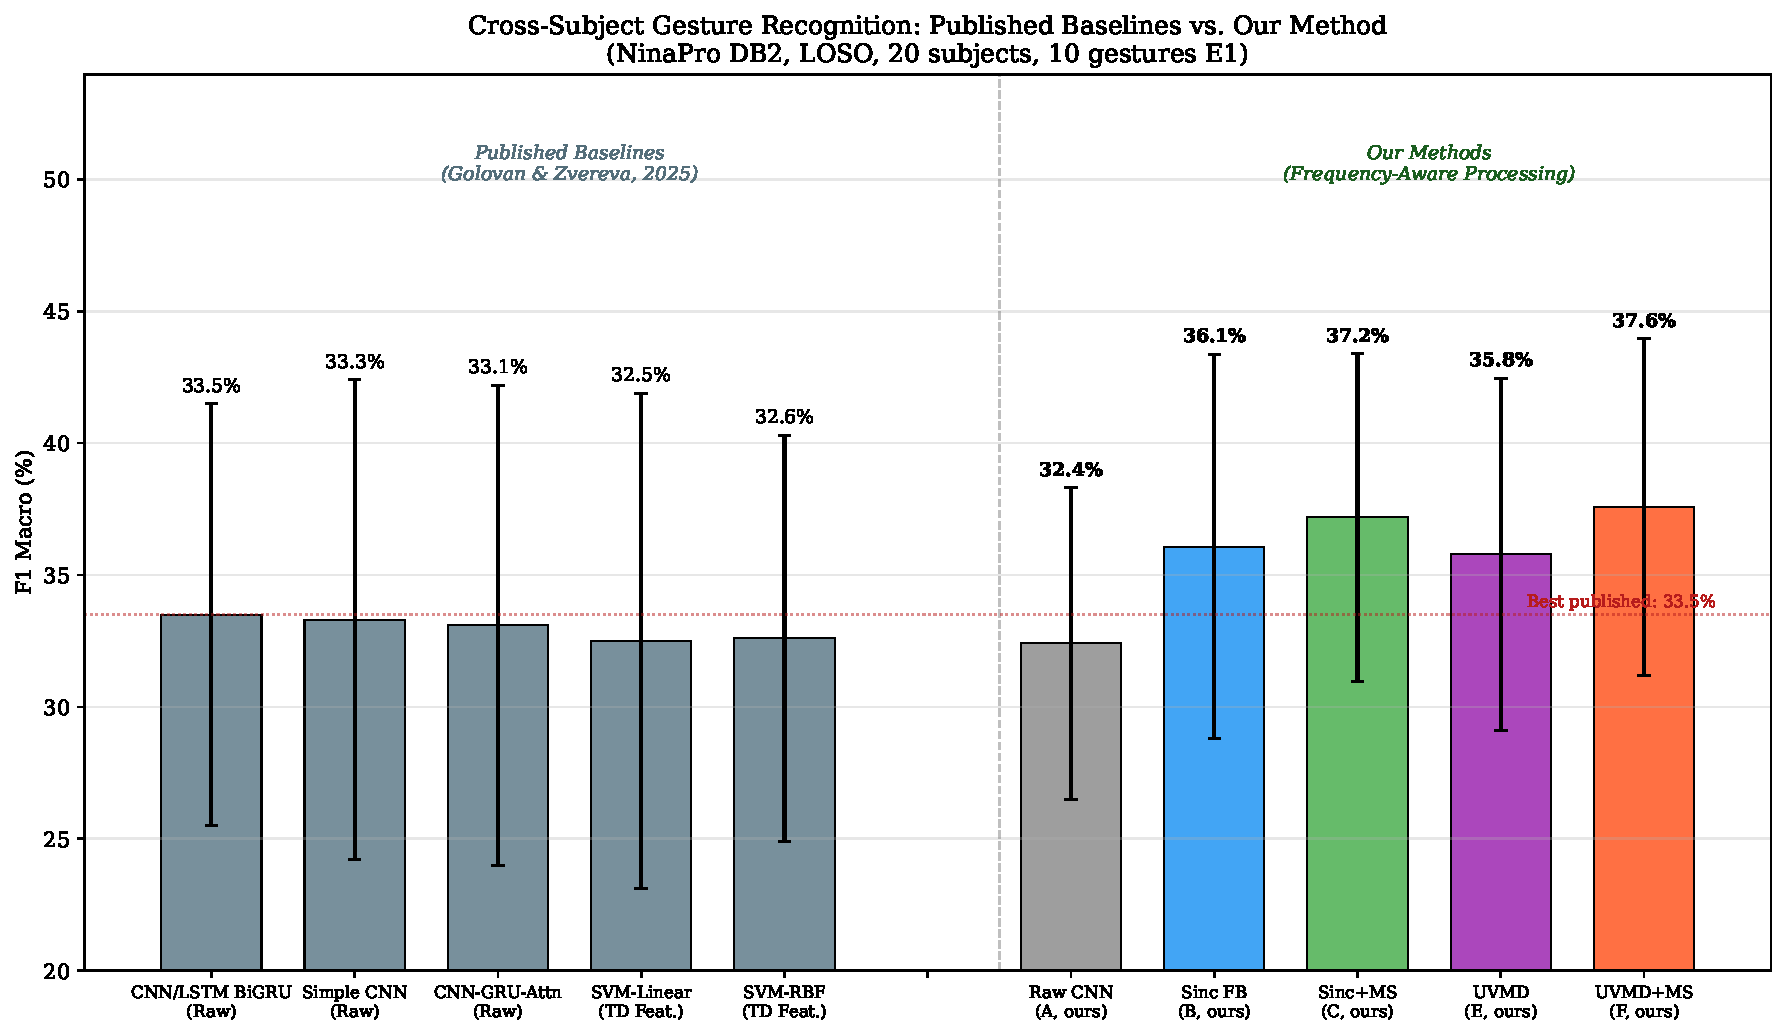
\includegraphics[width=\columnwidth]{fig_benchmark_comparison.pdf}
\caption{Сравнение с опубликованными бейзлайнами (серые) и вариантами нашего конвейера (цветные). Пунктирная линия: лучший опубликованный результат (33,5\%). Каждый вариант последовательно добавляет компоненты: декомпозиция, \mixstyle{}, обучаемый фронтенд.}
\label{fig:benchmark_bar}
\end{figure}

\subsection{Кому помогает \mixstyle{}?}

\Cref{fig:mixstyle_corr} показывает, что выигрыш от \mixstyle{} отрицательно коррелирует с базовым F1 для Sinc-фронтенда ($r$\,=\,$-$0,56, $p$\,=\,0,01): слабые субъекты выигрывают больше, сильные~--- меньше.
Это предполагает, что \mixstyle{} действует как регуляризатор, помогая прежде всего субъектам, чьи сигналы наиболее отклоняются от обучающего распределения.

\begin{figure}[t]
\centering
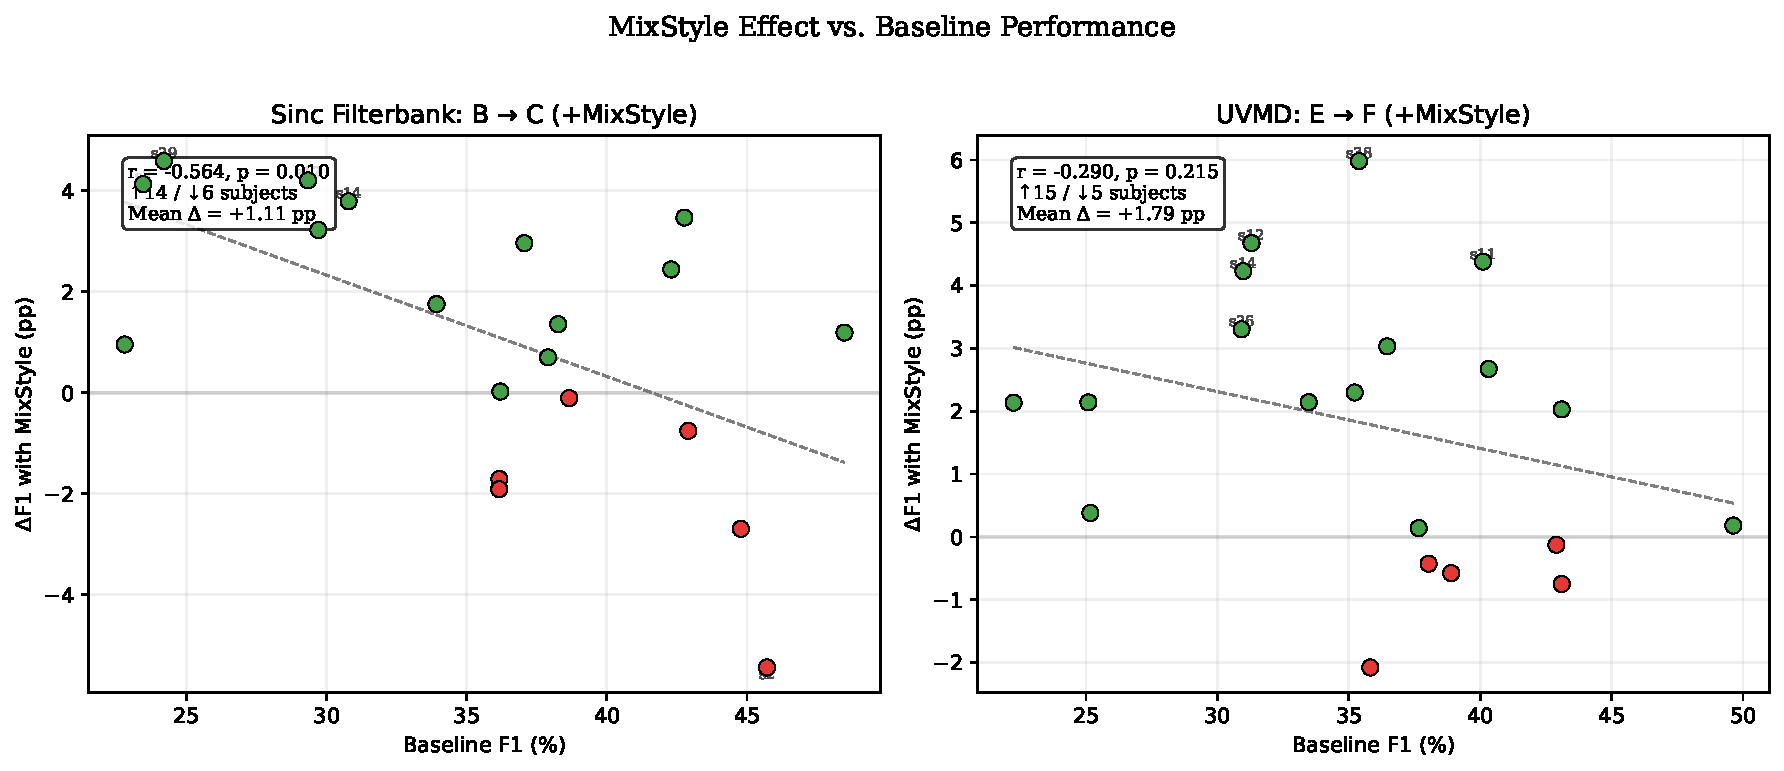
\includegraphics[width=\columnwidth]{fig_mixstyle_delta_correlation.pdf}
\caption{Пер-субъектный прирост F1 от \mixstyle{} vs. базовый F1. Слева: Sinc FB (B$\to$C), значимая отрицательная корреляция. Справа: \uvmd{} (E$\to$F), аналогичный тренд.}
\label{fig:mixstyle_corr}
\end{figure}

% ======================================================================
%  VII. АНАЛИЗ И ОБСУЖДЕНИЕ
% ======================================================================
\section{Обсуждение}
\label{sec:discussion}

\subsection{Центральный вывод: частотная селективность, а не глобальная инвариантность}

Совокупность результатов указывает на один ключевой вывод: \textbf{в пЭМГ субъект-инвариантность достигается не через глобальную нормализацию и не через разделение контента и стиля, а через частотно-селективную обработку, где низкочастотные полосы сохраняются, а высокочастотные~--- нормализуются или рандомизируются}.

Это подтверждается с трёх независимых сторон:
\begin{itemize}
    \item \emph{Аналитически}: спектральный анализ показывает десятикратный градиент межсубъектной вариабельности от низких к высоким частотам, при этом отношение Фишера движется в противоположном направлении.
    \item \emph{Через обучение}: адаптивный \mixstyle{} и SCG-Net, оптимизированные только по классификационной потере, независимо обучают монотонные градиенты параметров, воспроизводящие аналитическое наблюдение.
    \item \emph{Через отрицательные результаты}: глобальные подходы~--- равномерная IN ($-$7--8,5\pp{}), состязательное разделение ($-$2,6--4,3\pp{})~--- разрушают информацию о жестах, потому что амплитудный паттерн по 12~электродам одновременно кодирует жест \emph{и} физиологию субъекта.
\end{itemize}

Различие между аугментацией и удалением стиля также согласуется с этим выводом: \mixstyle{} (интерполяция статистик) сохраняет структуру распределения и увеличивает разнообразие обучения, тогда как SCG-Net и IN (удаление статистик) менее эффективны, даже будучи частотно-селективными.

\subsection{Конфаунд размера батча}
\label{sec:batchsize}

Ранние эксперименты использовали batch\_size\,=\,64, абляция~--- 512.
Абсолютные значения F1 различаются между сериями (напр., Raw CNN: 34,9\% при bs=64 vs. 32,4\% при bs=512), поэтому результаты разных серий \emph{не сопоставимы} напрямую.
Для проверки робастности мы воспроизвели лучший вариант (\uvmd{}+\mixstyle{}) при bs=64: 37,69\%\,$\pm$\,6,85~--- статистически не отличается от результата при bs=512 (37,58\%\,$\pm$\,6,39; Уилкоксон $p$\,=\,0,67).

\subsection{Ограничения}
\begin{enumerate}
    \item \textbf{Один датасет и упражнение.} Все результаты на NinaPro DB2 E1 (10~жестов, 12~каналов, 2000\,Гц). Генерализация на другие базы и аппаратуру не проверена.
    \item \textbf{Подмножество субъектов.} 20 из 40 доступных субъектов.
    \item \textbf{Неоднозначное свидетельство для \mixstyle{}.} Конфирматорный эффект только на \uvmd{}-фронтенде; на Sinc~--- разведочный.
    \item \textbf{Дескриптивный статус H8.} Градиент обученных параметров~--- наблюдение, а не контролируемый эксперимент.
    \item \textbf{Узкое сравнение SCG-Net.} Не сравнивается с другими архитектурами доменной генерализации (DANN, CORAL, DRO).
    \item \textbf{Новизна.} Декомпозиция и \mixstyle{}~--- устоявшиеся методы; наш вклад~--- их побандовая комбинация для пЭМГ.
\end{enumerate}

% ======================================================================
%  VIII. ЗАКЛЮЧЕНИЕ
% ======================================================================
\section{Заключение}
\label{sec:conclusion}

Межсубъектная вариабельность пЭМГ имеет выраженную частотную структуру.
Глобальные подходы к инвариантности~--- равномерная нормализация, состязательное разделение контента и стиля~--- разрушают информацию о жестах и ухудшают качество.
Частотно-селективная обработка, где низкочастотные полосы сохраняются, а высокочастотные нормализуются, устойчиво превосходит все проверенные альтернативы.

Конвейер, реализующий эту идею~--- декомпозиция на четыре поддиапазона + побандовый \mixstyle{}~--- достигает 37,7\% macro-F1 на NinaPro~DB2 (20~субъектов, LOSO) по сравнению с опубликованным бейзлайном 33,5\%, при этом декомпозиция обеспечивает основной вклад (+3,7\pp{}), а аугментация стилей~--- дополнительный (+1,1--1,8\pp{}).
Три независимых свидетельства~--- спектральный анализ, обученные параметры адаптивного \mixstyle{} и почти бинарный гейт SCG-Net~--- согласованно указывают на частотно-зависимую структуру вариабельности.

Результаты получены на одном датасете и требуют валидации на других бенчмарках пЭМГ.
В рамках этих ограничений центральный вывод прост: в сигналах пЭМГ субъект-инвариантность следует строить \emph{частотно-селективно}, а не глобально.

% ======================================================================
%  ЛИТЕРАТУРА
% ======================================================================
\bibliographystyle{IEEEtran}
\begin{thebibliography}{99}

\bibitem{atzori2016deep}
M.~Atzori \etal, ``Deep learning with convolutional neural networks applied to electromyography data: A resource for the classification of movements for prosthetic hands,'' \textit{Front. Neurorobot.}, vol.~10, 2016.

\bibitem{atzori2014electromyography}
M.~Atzori \etal, ``Electromyography data for non-invasive naturally-controlled robotic hand prostheses,'' \textit{Sci. Data}, vol.~1, p.~140053, 2014.

\bibitem{farina2014extraction}
D.~Farina \etal, ``The extraction of neural information from the surface EMG for the control of upper-limb prostheses: emerging avenues and challenges,'' \textit{IEEE Trans. Neural Syst. Rehabil. Eng.}, vol.~22, no.~4, pp.~797--809, 2014.

\bibitem{saponas2009enabling}
T.~S.~Saponas \etal, ``Enabling always-available input with muscle-computer interfaces,'' in \textit{Proc. UIST}, 2009.

\bibitem{campbell2020current}
E.~Campbell \etal, ``Current trends and confounding factors in myoelectric control: Limb position and contraction intensity,'' \textit{Sensors}, vol.~20, no.~6, 2020.

\bibitem{cote2019deep}
U.~C\^{o}t\'{e}-Allard \etal, ``Deep learning for electromyographic hand gesture signal classification using transfer learning,'' \textit{IEEE Trans. Neural Syst. Rehabil. Eng.}, vol.~27, no.~4, pp.~760--771, 2019.

\bibitem{du2017surface}
Y.~Du \etal, ``Surface EMG-based inter-session gesture recognition enhanced by deep domain adaptation,'' \textit{Sensors}, vol.~17, no.~3, 2017.

\bibitem{phinyomark2012feature}
A.~Phinyomark \etal, ``Feature reduction and selection for EMG signal classification,'' \textit{Expert Syst. Appl.}, vol.~39, no.~8, pp.~7420--7431, 2012.

\bibitem{golovan2025benchmark}
К.~Голован, И.~Зверева, ``Воспроизводимый бенчмарк для межсубъектного распознавания жестов кисти по сигналам пЭМГ,'' 2025.

\bibitem{dragomiretskiy2014variational}
K.~Dragomiretskiy, D.~Zosso, ``Variational mode decomposition,'' \textit{IEEE Trans. Signal Process.}, vol.~62, no.~3, pp.~531--544, 2014.

\bibitem{ravanelli2018speaker}
M.~Ravanelli, Y.~Bengio, ``Speaker recognition from raw waveform with SincNet,'' in \textit{Proc. SLT}, 2018.

\bibitem{zhou2021mixstyle}
K.~Zhou \etal, ``Domain generalization with MixStyle,'' in \textit{Proc. ICLR}, 2021.

\bibitem{hudgins1993new}
B.~Hudgins, P.~Parker, R.~N.~Scott, ``A new strategy for multifunction myoelectric control,'' \textit{IEEE Trans. Biomed. Eng.}, vol.~40, no.~1, pp.~82--94, 1993.

\bibitem{englehart2003robust}
K.~Englehart, B.~Hudgins, ``A robust, real-time control scheme for multifunction myoelectric control,'' \textit{IEEE Trans. Biomed. Eng.}, vol.~50, no.~7, pp.~848--854, 2003.

\bibitem{scheme2011electromyogram}
E.~Scheme, K.~Englehart, ``Electromyogram pattern recognition for control of powered upper-limb prostheses: State of the art and challenges for clinical use,'' \textit{J. Rehabil. Res. Dev.}, vol.~48, no.~6, pp.~643--659, 2011.

\bibitem{pizzolato2017comparison}
S.~Pizzolato \etal, ``Comparison of six electromyography acquisition setups on hand movement classification tasks,'' \textit{PLoS ONE}, vol.~12, no.~10, e0186132, 2017.

\bibitem{zhai2017self}
X.~Zhai \etal, ``Self-recalibrating surface EMG pattern recognition for neuroprosthesis control based on convolutional neural network,'' \textit{Front. Neurosci.}, vol.~11, 379, 2017.

\bibitem{wei2019multistream}
W.~Wei \etal, ``A multi-stream convolutional neural network for sEMG-based gesture recognition in muscle-computer interface,'' \textit{Pattern Recognit. Lett.}, vol.~119, pp.~131--138, 2019.

\bibitem{ketyko2019domain}
I.~Ketyk\'{o}, F.~Kov\'{a}cs, K.~Z.~Varga, ``Domain adaptation for sEMG-based gesture recognition with recurrent neural networks,'' in \textit{Proc. IJCNN}, 2019.

\bibitem{huang1998empirical}
N.~E.~Huang \etal, ``The empirical mode decomposition and the Hilbert spectrum for nonlinear and non-stationary time series analysis,'' \textit{Proc. R. Soc. Lond. A}, vol.~454, pp.~903--995, 1998.

\bibitem{rehman2010multivariate}
N.~Rehman, D.~P.~Mandic, ``Multivariate empirical mode decomposition,'' \textit{Proc. R. Soc. A}, vol.~466, pp.~1291--1302, 2010.

\bibitem{englehart1999wavelet}
K.~Englehart \etal, ``Classification of the myoelectric signal using time-frequency based representations,'' \textit{Med. Biol. Eng. Comput.}, vol.~37, no.~4, pp.~526--532, 1999.

\bibitem{phinyomark2018emg_frequency}
A.~Phinyomark, E.~Scheme, ``EMG pattern recognition in the era of big data and deep learning,'' \textit{Big Data Cogn. Comput.}, vol.~2, no.~3, 21, 2018.

\bibitem{borra2020sincnet_eeg}
D.~Borra \etal, ``Interpretable and lightweight convolutional neural network for EEG decoding: Application to movement execution and imagination,'' \textit{Neural Netw.}, vol.~129, pp.~55--74, 2020.

\bibitem{ioffe2015batch}
S.~Ioffe, C.~Szegedy, ``Batch normalization: Accelerating deep network training by reducing internal covariate shift,'' in \textit{Proc. ICML}, 2015.

\bibitem{ulyanov2016instance}
D.~Ulyanov, A.~Vedaldi, V.~Lempitsky, ``Instance normalization: The missing ingredient for fast stylization,'' \textit{arXiv:1607.08022}, 2016.

\bibitem{huang2017adain}
X.~Huang, S.~Belongie, ``Arbitrary style transfer in real-time with adaptive instance normalization,'' in \textit{Proc. ICCV}, 2017.

\bibitem{sagawa2020distributionally}
S.~Sagawa \etal, ``Distributionally robust neural networks for group shifts: On the importance of regularization for worst-case generalization,'' in \textit{Proc. ICLR}, 2020.

\bibitem{arjovsky2019invariant}
M.~Arjovsky \etal, ``Invariant risk minimization,'' \textit{arXiv:1907.02893}, 2019.

\bibitem{ganin2016domain}
Y.~Ganin \etal, ``Domain-adversarial training of neural networks,'' \textit{J. Mach. Learn. Res.}, vol.~17, no.~59, pp.~1--35, 2016.

\bibitem{wang2022generalizing}
J.~Wang \etal, ``Generalizing to unseen domains: A survey on domain generalization,'' \textit{IEEE Trans. Knowl. Data Eng.}, vol.~35, no.~8, pp.~8052--8072, 2023.

\bibitem{holm1979simple}
S.~Holm, ``A simple sequentially rejective multiple test procedure,'' \textit{Scandinavian J. Statistics}, vol.~6, no.~2, pp.~65--70, 1979.

\end{thebibliography}

\end{document}
